\documentclass[Lau, oneside]{sapthesis}%remove "english" for a thesis written in Italian
%Bachelor's (laurea triennale) thesis : Lau
\usepackage[english]{babel} %use this package for a thesis written in Italian
\usepackage[utf8]{inputenx}
\usepackage{indentfirst}
\usepackage{microtype}
\usepackage{amsmath}
\usepackage{amssymb}
%\usepackage{chemformula}
%\usepackage{setspace}
%\usepackage{yfonts,color}
%\usepackage{siunitx}
%\usepackage{comment}
%\usepackage{multirow}
%\usepackage{varioref}
%\usepackage[bottom]{footmisc}
%\usepackage{wrapfig}
\usepackage{float}
%\usepackage{type1cm}
\usepackage{titlesec}
\usepackage{lettrine}
\usepackage{caption}
\usepackage{subcaption}
\usepackage{listings}
\lstdefinelanguage{SymQEMU}{
    morekeywords={movi_i64, add_i64, ext32u_i64, call, void, ZMMReg, float, SymExpr, uint8_t, if, else, class, public, ExprRef, protected, std, string, const, return, z3, expr, bool, Z3_ast, Z3_sort, override, int, UINT32, double},
    sensitive=false, % keywords are not case-sensitive
}
\lstdefinelanguage{SymQEMU2}{
    morekeywords={movi_i64, add_i64, ext32u_i64, call, void, ZMMReg, float, SymExpr, uint8_t, if, else, class, public, ExprRef, protected, std, string, const, return, z3, bool, Z3_ast, Z3_sort, override, int},
    sensitive=false, % keywords are not case-sensitive
}
\linespread{0.9}
%\usepackage{chngcntr}
\usepackage[nottoc, notlof, notlot]{tocbibind}
%\onehalfspacing
%\counterwithout{footnote}{chapter}
\usepackage{hyperref}
\hypersetup{		
			colorlinks=true,
			linkcolor=red,
                        linktoc=page,
			anchorcolor=black,
			citecolor=red,
			urlcolor=blue,
			pdftitle={Analysis of fuzz testing campaigns (temp)},
			pdfauthor={Matteo Sabatini},
			pdfkeywords={thesis, sapienza, roma, university}
}

\title{Analysis of fuzz testing campaigns (temp)}
\author{Matteo Sabatini}
\IDnumber{1794627}
\course{Cybersecurity}
\courseorganizer{Facolt\`a di Ingegneria dell'informazione, informatica e statistica}
\submitdate{2023/2024}
\copyyear{2024}
\advisor{(Prof. ??) Daniele Cono D'Elia}
\authoremail{sabatini.1794627@studenti.uniroma1.it}
\examdate{(??)}
\examiner{Prof. ??} \examiner{Prof. ??} \examiner{Prof. ??}  \examiner{Prof. ??}  \examiner{Prof. ??} \examiner{Prof. ??}  \examiner{Prof. ??}
\thesistype{Master thesis}

%we refer to http://ctan.mirrorcatalogs.com/macros/latex/contrib/sapthesis/sapthesis-doc.pdf for an exhaustive description of the sapthesis documentclass.


\begin{document}


\setlength{\parindent}{0pt}    %elimina l'indentazione leggermente a destra per ogni nuovo capitolo/paragrafo
\frontmatter
\maketitle

\begin{abstract}
???
\newline \newline
\end{abstract}




\tableofcontents


\titleformat{\chapter}[display]  
{\normalfont\Huge\bfseries}{\chaptertitlename\ \thechapter}{20pt}{\huge}  
\titlespacing{\chapter}{0pt}{0pt}{0pt}  

\mainmatter
\chapter{Introduzione}
\ \\
Tra le varie tecniche di program analysis attualmente esistenti, l'\textit{esecuzione simbolica (symbolic execution)} si è affermata negli ultimi tempi come una delle strategie che fornisce la più completa analisi del codice studiato.
\newline
Il concetto alla base è riscrivere l'esecuzione del programma come una lunga formula matematica, la cui complessità dipende dalla struttura del codice, ed individuare possibilmente delle soluzioni che siano in grado di rendere la formula vera o falsa.
\newline \newline
La base dell'analisi simbolica sono i \textit{simboli}, che nel programma corrispondono a tutti quegli input non conosciuti a tempo di compilazione (es. input utente, lettura da file, etc.), e sono le variabili incognite della formula in cui bisognerà andare a sostituire dei valori per il calcolo della soddisfacibilità.
\newline \newline
Generalmente, l'esecuzione simbolica viene utilizzata per generare input in grado di esercitare i diversi percorsi di esecuzione di un programma.
\newline
Risulta tuttavia ovvio che analizzare tutti i possibili percorsi di esecuzione di un dato programma può facilmente diventare proibitivo in termini di complessità e tempo impiegato per la risoluzione, soprattutto se con riferimento a programmi reali di uso comune, e questo è uno dei principali compromessi con cui ha a che fare l'esecuzione simbolica.
\newline
Ogni volta che all'interno di un programma è presente la verifica di una condizione, l'analisi si divide in due universi separati sulla seguente ipotesi: una procederà supponendo la condizione verificata, l'altra supponendola non verificata.
\newline
Inoltre, un programma potrebbe utilizzare dei controlli estremamente specifici per garantirne la sicurezza, come ad esempio dei checksum, oppure avere delle funzionalità che sfruttano librerie esterne al codice o altri blocchi non conosciuti dall'esecutore.
\newline \newline
Ne segue quindi che l'analisi di un programma reale rappresenta una delle principali sfide e limitazioni a cui è soggetta \textit{symbolic execution}, e che tutt'ora è oggetto di studio da parte della comunità scientifica.
\newline \newline
Per cercare di risolvere i problemi sopra descritti sono state inventate altre tecniche direttamente derivanti dall'approccio puramente simbolico, tra cui \textit{concolic execution}: partendo da un insieme di input interessanti forniti dall'utente, l'esecuzione concreta del codice "guida" quella simbolica nel percorso da seguire, fino ad arrivare ad una delle possibili formule finali che verrà valutata per generare altri input interessanti.
\newline
Basandosi quindi sull'effettivo comportamento assunto dal programma su input prestabiliti, questa strategia punta a rendere più efficiente e veloce l'analisi, eliminando il calcolo di vincoli troppo complessi e diminuendo il numero di formule da studiare contemporaneamente.
\newline
I percorsi alternativi non esplorati durante una singola esecuzione del codice vanno però considerati, 
ed è compito dell'esecutore generare nuovi input interessanti in modo tale che, nelle successive esecuzioni, questi verranno attraversati.


\newpage
Gli esecutori simbolici attualmente esistenti forniscono supporto alle operazioni più semplici e comuni utilizzate durante la programmazione, ma in pochi consentono di ragionare simbolicamente sui numeri in virgola mobile.
\newline \newline
L'obiettivo di questa tesi è stato inizialmente studiare il funzionamento dell'esecutore concolico SymQEMU, basato a sua volta su componenti sviluppati nei progetti SymCC e QSYM: esso analizza programmi binari e costruisce formule simboliche durante l'esecuzione, interrogando un SMT solver per generare nuovi input concreti.
\newline 
Successivamente, è stato integrato in SymQEMU il supporto alla costruzione di formule simboliche in grado di rappresentare:
\begin{itemize}
    \item valori floating-point
    \item operazioni matematiche di base tra floating-point
    \item operazioni di confronto tra floating-point
\end{itemize}
Per fare ciò è stato necessario inserire in SymQEMU delle funzioni che associano un'espressione simbolica alle istruzioni x86 e x86\_64 interessate dalle operazioni sopraindicate e, successivamente, andare a modificare il runtime di SymQEMU per consentire all'esecutore di generare le corrette formule comprensibili ad un SMT solver.
\newline \newline \newline
Nella prima parte dell'elaborato viene fatta una descrizione di \textit{symbolic execution} e \textit{concolic execution}, analizzandone rispettivamente le caratteristiche ed i punti di forza e di debolezza, e fornendo anche una panoramica generale sui framework utilizzati.
\newline \newline
Successivamente vengono dati richiami sulla notazione binaria, introdotta la notazione in virgola mobile limitandosi ai formati di interesse per questo studio, come vengono rappresentati questi numeri reali in memoria e la loro gestione da parte della CPU e della FPU.
\newline \newline
Infine, viene data un'ampia spiegazione delle modifiche apportate a SymQEMU, inclusi i componenti interni derivati da SymCC e QSYM.
\newline
Per mostrare il corretto funzionamento delle modifiche introdotte, vengono presentati diversi esempi pratici ed i risultati ottenuti in seguito al lavoro svolto.





\chapter{Symbolic Execution}
\ \\
\textit{Symbolic Execution} è una tecnica di program analysis utilizzata per verificare il comportamento di un programma al variare degli input e, per quanto la sua efficacia sia estremamente elevata e indiscutibile, bassa velocità di esecuzione e ridotta scalabilità sono le principali limitazioni che la affliggono.
\newline \newline
L'esecuzione simbolica si basa sull'analisi di un codice in ingresso, binario o sorgente a seconda di come è implementata la tecnica, il quale eseguirà un certo numero di istruzioni: compito dell'esecutore è cercare di rappresentare il codice iniziale come un'unica formula matematica.
\newline
I principali componenti delle formule sono proprio le variabili che le costituiscono, e queste prendono il nome di \textit{simboli}: essi rappresentano degli input arbitrari immessi dall'utente all'inizio del programma, quindi noti solo a tempo di esecuzione, e su cui verranno eseguite operazioni matematiche e imposte delle condizioni di validità.
\newline \newline
Riuscire però a rappresentare anche solo poche righe di programma come una formula matematica non è banale, e la complessità di un'espressione crescerebbe esponenzialmente se venissero considerati tutti i possibili modi in cui può svolgersi la sua risoluzione.
\newline
La completezza nell'analisi del codice è quindi contrastata dall'enorme complessità nelle formule generate e l'elevato tempo richiesto per provare a calcolarne la loro soddisfacibilità: per questo motivo la pura esecuzione simbolica viene spesso affiancata da strategie che, ad esempio, tentano di alleggerire le formule effettuando semplificazioni o calcoli parziali del risultato.
\newline \newline
Quest'ultimo punto in particolare costituisce uno dei principali "bottleneck" dell'esecuzione simbolica: durante la costruzione di un'espressione simbolica, ed in particolare nell'analisi dei costrutti condizionali, vengono imposte delle condizioni sui simboli che occorrerà valutare.
\newline
Nella verifica della soddisfacibilità, ogni qualvolta si incontri una di queste condizioni, l'analisi subisce una divisione: un percorso prosegue il calcolo supponendo la condizione verificata, l'altro supponendola non verificata.
\newline
Risulta quindi ovvio che, data una formula apparentemente semplice ma ricca di condizioni sui dati, l'analisi potrebbe suddividersi talmente tante volte da esplodere (\textit{path explosion}) e rendere impossibile il calcolo finale.
\newline \newline
Con il passare degli anni sono stati sviluppati nuovi approcci ibridi all'esecuzione simbolica come ad esempio \textit{Concolic Execution}, in cui l'analisi simbolica viene semplificata tramite euristiche e calcoli parziali nelle formule.
\newline \newline
Nei paragrafi successivi verranno trattate nello specifico entrambe le tecniche, e successivamente fatta un'analisi dei framework utilizzati in questa tesi e delle loro caratteristiche.



\newpage
\section{Cosa è un esecutore simbolico}
Un \textit{esecutore simbolico} è un programma per l'analisi del software basato su un approccio puramente simbolico.
\newline \newline
Il lavoro compiuto consiste nell'analizzare singolarmente ogni istruzione presente nel codice, effettuando le operazioni richieste per consentirgli di proseguire nella sua esecuzione, ed al tempo stesso associare ad ognuna di esse una funzione che la rappresenti simbolicamente nella formula finale.
\newline
Ad un occhio attento il comportamento risulta essere molto simile a quello di un interprete, con l'aggiunta di uno strato intermedio di lavoro che è proprio la componente simbolica. 
\newline \newline
Un esecutore simbolico, in ogni momento, si basa su due informazioni:
\begin{itemize}
    \item la formula simbolica
    \item lo stato della memoria simbolica
\end{itemize}
La \textit{formula} viene generata a seguito della valutazione del codice in input al programma, rappresenta in modo matematico le istruzioni presenti all'interno di questo ed è il principale oggetto di studio dell'analisi.
\newline \newline
La \textit{memoria simbolica} tiene conto di tutti i simboli presenti all'interno della formula, delle condizioni imposte su di essi, delle eventuali operazioni che ne definiscono il valore in ogni stato ed è diversa per ogni percorso di esecuzione durante il calcolo della soddisfacibilità.
\newline \newline
Di seguito analizziamo in dettaglio alcuni aspetti rilevanti che impattano il ra-
gionamento simbolico su un programma.
\newline \newline \newline
\textbf{Accessi in memoria.}\ \ \ Un’enorme sfida nelle performance di un esecutore simbolico è rappresentata dal ragionare su accessi in memoria simbolici, ossia caratterizzati da un indirizzo di memoria dipendente dal valore di un input.
\newline
Tra i diversi approcci attualmente utilizzati per ragionare simbolicamente sugli accessi in memoria, citiamo il \textit{puramente simbolico} ed il \textit{parzialmente simbolico}.
\newline \newline
Nel massimo livello di astrazione, cioè \textit{puramente simbolico}, tutti gli indirizzi di memoria diventano dei simboli.
\newline
Questa scelta comporta la necessità di considerare tutti i possibili stati risultanti a seguito di un'operazione di lettura/scrittura di un indirizzo, ottenendo così un'accurata descrizione del comportamento che il programma potrebbe assumere.
\newline
Bisogna però notare che analizzare tutti questi stati potrebbe facilmente far esplodere il numero di percorsi, quindi un approccio di questo tipo diventerebbe particolarmente costoso nei programmi reali per via della sua scarsa scalabilità.
\newline \newline
Nel modello \textit{parzialmente simbolico} gli indirizzi vengono concretizzati se subiscono scritture e simbolizzati se subiscono letture, supponendo però che il numero di dati letti/scritti sia sufficientemente piccolo.
\newline
Per \textit{concretizzazione} si intende utilizzare un singolo valore possibile concreto per la formula sotto analisi, consentendo di ridurre il numero dei possibili stati in seguito ad una lettura/scrittura e semplificare le formule data ora la presenza di valori costanti.


\newpage
Affidarsi a valori concreti può consentire di ottenere formule più facili e quindi risolvibili in tempi minori, ma anche la possibilità di non esplorare percorsi che dipendono da valori estremamente specifici di tali indirizzi concretizzati.
\newline
Questa tecnica si basa su un compromesso tra l'espressività della formula, ora composta da molteplici valori concreti, e la possibile perdita di informazioni risultanti da un'analisi meno completa.
\newline \newline \newline
\textbf{Percorsi di esecuzione.}\ \ \ L’esecuzione simbolica cerca di generare input in grado di esplorare esaustivamente i vari percorsi di esecuzione di un programma.
\newline
Da un punto di vista reale, tenere conto di tutti i possibili percorsi di esecuzione durante un'analisi richiederebbe tempistiche proibitive, pertanto vengono applicate delle euristiche che consentono di esplorare i vari percorsi cercando di considerare quelli più "interessanti".
\newline \newline
Alcune delle tecniche maggiormente applicate sono la \textit{Depth-First Search} (DFS) e la \textit{Breadth-First Search} (BFS):
\begin{itemize}
    \item la DFS è una ricerca in \textit{profondità}, ovvero in cui un percorso viene esplorato il più possibile e poi si risale fino al primo inesplorato per ripetere l'operazione
    \item la BFS è una ricerca in \textit{ampiezza}, ovvero in cui ogni percorso viene analizzato contemporaneamente con gli altri, consentendo subito di scoprire comportamenti interessanti
\end{itemize}
Ovviamente, ognuna di esse ha dei vantaggi e degli svantaggi.
\newline
La DFS, ad esempio, è molto utile nei casi in cui la memoria a disposizione sia scarsa, però potrebbe diventare estremamente costosa se il percorso analizzato fosse ricco di cicli o chiamate ricorsive.
\newline
La BFS, d'altro canto, è molto più dispendiosa in termini di memoria data l'esplorazione parallela di molteplici percorsi, ma consente anche di scoprire nei primi stage dell'analisi eventuali comportamenti interessanti da parte del codice.
\newline \newline
Un'altra strategia molto adottata è la \textit{random path selection}, che nel corso degli ultimi anni è stata fra quelle maggiormente studiate e raffinate.
\newline
Il suo obiettivo è ottenere la massima \textit{copertura del codice}, cioè l'analisi del maggior numero possibile di righe di programma prima di cambiare percorso, e per farlo si basa su delle euristiche: queste assegnano ai vari percorsi di esecuzione un valore chiamato peso (\textit{weight}), che rappresenta quanto sono interessanti, ed un valore che indica la frequenza con cui vengono esplorati durante l'analisi complessiva del codice.
\newline
Così facendo si riesce anche ad ovviare alla \textit{starvation} causata dai percorsi troppo complessi, portando l'analisi in favore di quelli più semplici o interessanti.
\newline \newline
È importante però ricordare che, in fase di sviluppo dell'esecutore, la strategia scelta è generalmente ottimizzata per raggiungere dei risultati specifici: alcune mirano a massimizzare il numero di istruzioni distinte analizzate, altre ad analizzare i percorsi meno ricorrenti nell'analisi o con maggiori errori, altre ancora ad analizzare un percorso specifico piuttosto che altri o concentrarsi sulla ricerca di uno specifico bug.
\newline \newline
Ne segue quindi che la scelta della strategia utilizzata per l'analisi del codice riveste un ruolo fondamentale verso l'obiettivo finale, ed euristiche diverse possono portare alla scoperta di bug differenti.


\newpage
Problema principale di cui soffrono queste strategie è \textit{path explosion}.
\newline
Nei programmi reali, il numero di possibili percorsi di esecuzione da esplorare in seguito alla divisione dell'analisi può facilmente aumentare esponenzialmente, e tenerne traccia di tutti potrebbe provocare enormi costi in termini di tempo e spazio utilizzato.
\newline
Ad esempio, un ciclo all'interno di un programma viene visto come un costrutto \textit{if-else} 
su cui è necessario dividere l'analisi, così come le chiamate a funzione (specialmente se ricorsive) contribuiscono a generare molteplici possibili esecuzioni del codice.
\newline \newline \newline
\textbf{Prestazioni di un esecutore simbolico.} \ \ In termini di performance, un esecutore simbolico si basa su tre principi:
\begin{itemize}
    \item \textbf{impiego delle risorse}: l'esecutore deve essere in grado di procedere nell'analisi per un tempo indefinito rimanendo sempre nei limiti delle risorse messe a disposizione, dove spesso la più critica è proprio la memoria
    \item \textbf{analisi smart}: i risultati di precedenti analisi devono essere riutilizzati il più possibile per aumentare l'efficienza, soprattutto nel caso di risoluzione delle formule per evitare il calcolo della soddisfacibilità di condizioni già valutate
    \item \textbf{overhead}: evitare di resettare l'esecuzione di un programma nel corso dell'analisi, così da non ripetere istruzioni già analizzate e dal carico computazionale potenzialmente non indifferente
\end{itemize}
Un esecutore simbolico ideale riuscirebbe ad essere ottimizzato in tutti e tre i punti sopraindicati, ma nel mondo reale c'è bisogno di un trade-off fra performance e completezza dell'analisi.
\newline
Tutt'ora, il tempo di esecuzione impiegato per un'analisi completa e approfondita del codice è uno dei principali compromessi dell'esecuzione simbolica, ed è per questo motivo che spesso bisogna rinunciare alla precisione per rientrare in tempi ragionevoli.
\newline \newline \newline
\textbf{Completezza dell'analisi.}\ \ Infine, una delle principali sfide di questa tecnica di analisi è l'impossibilità di simbolizzare l'intera esecuzione di un codice.
\newline
Un programma reale fa spesso uso di chiamate esterne ad esso nella sua esecuzione, come ad esempio syscall o metodi di librerie, e l'esecutore simbolico non è in grado di tracciare tutte le operazioni che avvengono nel \textit{software stack} e quindi gestire i side-effect eseguiti al di fuori del codice in input.
\newline
Inoltre, condizioni estremamente specifiche sui simboli (es. checksum, sistemi non lineari, trigonometria, etc.)  non possono essere gestite per via dell'enorme complessità e del tempo che potrebbe richiedere la loro risoluzione.





\newpage
\section{Importanza dell'SMT solver}
Durante il lavoro di analisi compiuto dall'esecutore simbolico, l'ultima fase è affidata ad un programma esterno che, nel nostro caso, si tratta di un \textit{Satisfiability Modulo Theories solver} (SMT solver).
\newline
Esso ha il compito di verificare la soddisfacibilità delle formule e di assegnare ai simboli un possibile set di valori concreti che saranno utilizzati per dimostrare la possibilità di risoluzione o meno. 
\newline \newline
I problemi di calcolo della soddisfacibilità non sono sempre risolvibili in tempi polinomiali, e per questo bisogna fare ricorso a delle approssimazioni.
\newline
Punto di forza di questi SMT solver è quello di riuscire a generalizzare il problema SAT, basandosi su delle euristiche, e concentrandosi sulla risoluzione delle componenti più lineari e semplici della formula.
\newline \newline
Questo passaggio costituisce uno dei principali ostacoli alla scalabilità degli esecutori simbolici, dato l'enorme tempo che potrebbe essere necessario per risolvere formule molto complesse, e anche qui è sempre presente il compromesso fra tempo impiegato e completezza dell'analisi.
\newline \newline
Una delle tecniche di ottimizzazione più usate, ed anche la più intuitiva, è la \textit{semplificazione dei constraints}, ovvero l'elaborazione parziale della formula effettuando delle operazioni di semplificazione come constant folding, applicazione delle proprietà dei campi matematici, sostituzione di istruzioni complesse con più istruzioni semplici, etc.
\newline
L'idea alla base è che una condizione complessa può essere suddivisa in diverse condizioni basilari, più facilmente risolvibili dall'SMT solver, ottenendo un minore tempo di calcolo per constraint.
\newline
Ad esempio, l'introduzione di un vincolo di uguaglianza su di un simbolo può diventare un'informazione molto importante, in quanto il nuovo valore concreto assegnato può essere subito usato per verificare le eventuali condizioni già presenti sul simbolo.
\newline \newline
Un'altra tecnica di ottimizzazione consiste nel riutilizzo di soluzioni già calcolate durante la risoluzione di altri constraints, eliminando l'overhead dovuto ad una computazione già eseguita.
\newline
Se durante l'analisi di un dato percorso dovessero essere presenti più constraints \textit{semanticamente equivalenti}, il risultato dovuto alla risoluzione del primo può essere memorizzato ed usato come prova o controprova della soddisfacibilità di un suo simile.
\newline \newline
Su quest'ultima idea si basa anche la strategia di raggruppamento dei constraints in \textit{insiemi}: se il vincolo più semplice in profondità non è soddisfacibile allora tutto l'insieme non è soddisfacibile, se invece il vincolo esterno più complesso è risolvibile allora lo saranno anche quelli più interni.
\newline \newline \newline
Nonostante l'indiscutibile importanza che hanno gli SMT solver nel finalizzare l'analisi simbolica, purtroppo non tutti i tipi di \textit{constraint} possono essere risolti e non tutte le formule possono essere semplificate e risolte in tempi ragionevoli.
\newline
Per affiancare l'enorme lavoro di elaborazione compiuto dal solver, spesso si utilizzano approcci ibridi che eseguono operazioni di semplificazione già durante l'analisi del codice.





\newpage
\section{Esempio: funzionamento di un esecutore simbolico}
Si consideri il seguente codice: l'obiettivo è determinare per quali valori in input la funzione fallisce, ovvero la condizione nell'\textit{assert}
(riga 8) non è verificata.
\newline
\begin{figure}[h]
\centering
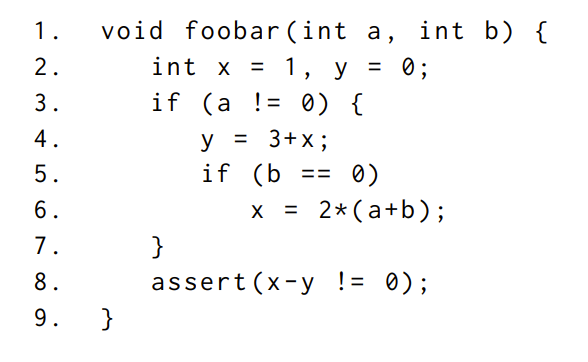
\includegraphics[scale=0.3]{foto/esempio_symbolic.png}
\caption{Quali sono i valori di $a$ e $b$ che fanno scattare l'assert? \cite{ref:survey}}
\label{fig:esempio_1}
\end{figure}
\newline
I parametri in ingresso alla funzione sono interi, aventi dimensione 4 byte e $2^{32}$ possibili valori, pertanto utilizzare un approccio casuale comporterebbe probabilità estremamente basse di individuazione della soluzione.
\newline
Piuttosto che utilizzare valori concreti, si utilizza un approccio che definisce le due variabili come \textbf{simboli} all'interno di una formula, il cui valore non è noto fino a quando non viene calcolata la soddisfacibilità.
\newline \newline
Supponendo di effettuare uno snapshot di un percorso durante l'analisi del codice, in ogni momento l'esecutore memorizza tre informazioni:
\begin{itemize}
    \item il prossimo \textit{statement} da valutare, ovvero la prossima istruzione da analizzare, e le operazioni che può eseguire sono assegnazioni, condizioni o salti
    \item lo stato della \textit{memoria simbolica}, dove ad ogni simbolo possono essere assegnati altri simboli o espressioni simboliche
    \item gli attuali \textit{path constraints}, ovvero il valore di verità di tutte le espressioni condizionali incontrate finora per arrivare in questo percorso
\end{itemize}
\ \\
Se lo \textit{statement} valutato è un'\textbf{assegnazione}, viene aggiornato lo stato simbolico del simbolo coinvolto nella \textit{memoria simbolica}, ed il nuovo valore assunto è un'espressione simbolica $e_{s}$.
\newline
Questa associazione viene rappresentata come $x \rightarrow e_s$, dove $e_s$ è ottenuta valutando l'espressione simbolica fino a quel particolare stato.
\newline \newline
Se lo \textit{statement} è un'istruzione \textbf{condizionale} allora l'analisi deve dividersi in due percorsi, uno in cui lo \textit{statement} è verificato ($s_{true}$) ed uno in cui non lo è ($s_{false}$).
\newline
I due nuovi stati generati procederanno in modo indipendente l'uno dall'altro, portando a due analisi diverse del codice.
\newline \newline
Se lo \textit{statement} è un \textbf{salto incondizionato}, lo stato avanza e salta direttamente alla nuova istruzione indicata.

\newpage
\begin{figure}
\makebox[\textwidth][c]{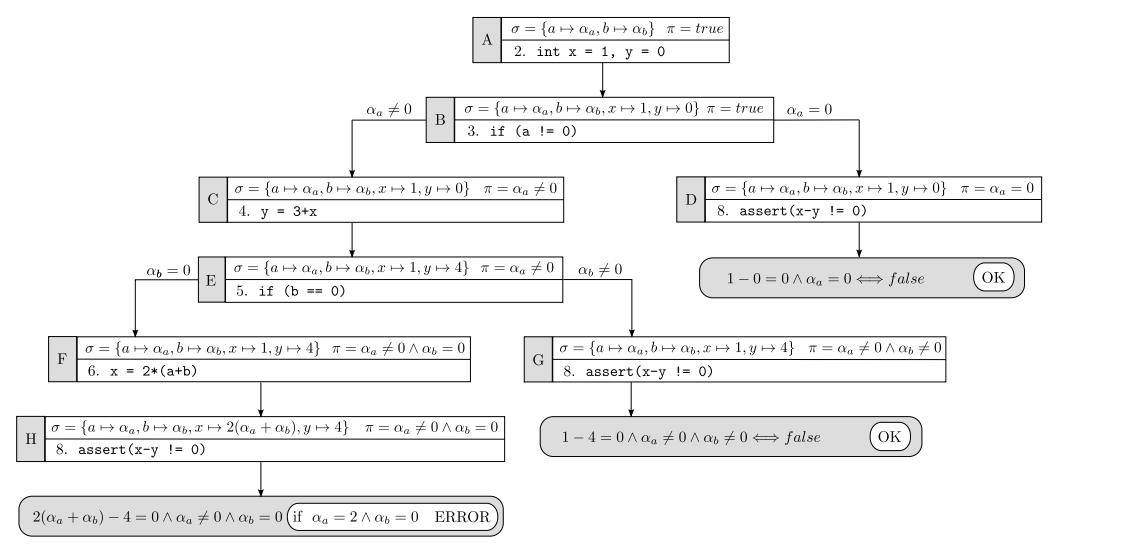
\includegraphics[width=0.9\paperwidth]{foto/albero_symbolic.png}}
\newline
\caption{Rappresentazione grafica del progresso nell'analisi simbolica del codice \ref{fig:esempio_1}. \cite{ref:survey}}{La prima riga di ogni stato rappresenta l'espressione simbolica fino a quel momento, la riga successiva il prossimo \textit{statement} da valutare.}
\label{fig:esempio_2}
\end{figure}
Come si nota dalla Figura (\ref{fig:esempio_2}), l'analisi simbolica può essere rappresentata come un albero.
\newline
Gli stati che hanno un solo figlio contengono \textit{statement} non condizionali, e pertanto sono proseguiti in modo lineare nell'analisi, mentre gli altri hanno incontrato qualche costrutto che ha imposto la divisione in due percorsi separati.
\newline \newline
Nello stato iniziale $A$ vengono definiti i nuovi simboli associati alle variabili $a$ e $b$ ed i \textit{path constraints} definiti per default a $true$.
\newline \newline
Nello stato $B$ si può vedere la valutazione dello \textit{statement} indicato in $A$, ovvero nell'espressione simbolica sono state aggiunte le variabili $x$ e $y$ in modo concreto poiché il loro valore era già conosciuto a tempo di compilazione.
\newline
Il suo \textit{statement} successivo però è un costrutto condizionale $if(a!=0)$, pertanto verranno a crearsi due nuovi stati che continueranno in modo indipendente l'analisi: lo stato $C$ in cui si è imposto $a\neq0$, e lo stato $D$ in cui invece $a=0$.
\newline \newline
Procedendo secondo la logica sopraindicata, si arriva agli stati finali $D$, $G$ e $H$.
\newline
Ognuno di essi ha un'espressione simbolica finale diversa, dimostrando appunto che ogni percorso procede in modo autonomo arrivando ad una propria conclusione.
\newline
Le seguenti espressioni sono quindi date in input all'SMT solver, che provvederà a verificarne la soddisfacibilità: in questo caso, mentre le espressioni simboliche generate in $D$ e $G$ sono sempre verificate, l'espressione in $H$ risulta non soddisfacibile (ad esempio) per $a=2$ e $b=0$.


\newpage
È importante notare che questi due valori generati dall'SMT solver non sono necessariamente gli unici che non la soddisfano, costituiscono soltanto una possibile coppia che andrebbe a creare problemi per la funzione studiata.
\newline \newline \newline
L'esempio appena mostrato è un codice di piccole dimensioni e di non elevata difficoltà, ma che riesce comunque a mostrare come \textit{symbolic execution} analizzi tutti i possibili svolgimenti del codice per poi studiarne il comportamento al variare degli input.
\newline
Nonostante l'approccio puramente simbolico sia virtualmente in grado di scoprire tutti i possibili input interessanti per un programma, tramite un'analisi estremamente approfondita del codice in input, l'applicazione di un ragionamento di questo tipo a situazioni reali comporta una serie di problematiche aggiuntive che in ambienti di test controllati possono essere trascurate.
\newline
Di seguito ne riportiamo alcune:
\begin{itemize}
    \item gestire simbolicamente lo stato della memoria in merito a puntatori, array, strutture dati o altri oggetti complessi, considerando la necessità di dover simbolizzare il concetto di indirizzo
    \item gestire simbolicamente le chiamate a funzioni attraverso i vari strati del \textit{software stack}, anche se tenere conto di tutti i possibili side-effect dovuti ad invocazione dei metodi delle librerie o syscalls risulta essere molto difficile se non impossibile
    \item codici estremamente lunghi e complessi potrebbero facilmente causare \textit{path explosion} e, nonostante l'esecutore sarebbe tecnicamente in grado di esplorare tutti i possibili percorsi, sicuramente non avverrebbe in un tempo ragionevole
    \item il calcolo della soddisfacibilità delle formule generate potrebbe dover ragionare su centinaia di variabili alla volta, costituendo un enorme ostacolo per l'efficienza e la velocità di esecuzione
\end{itemize}
\ \\
Per questo motivo sono stati introdotti nuovi approcci ibridi a \textit{symbolic execution}, come ad esempio \textit{concolic execution}.




\newpage
\section{Concolic Execution}
Un \textit{esecutore concolico} è uno dei tanti approcci ibridi all'esecuzione simbolica, dove simboli ed input concreti forniti dall'utente vengono usati insieme al fine di ottenere una maggiore velocità esecutiva e scalabilità nel codice.
\newline \newline
Il principale scopo dell'esecuzione concolica è quello di alleggerire il lavoro compiuto dall'esecutore simbolico, ad esempio nella risoluzione di constraints particolarmente specifici o nell'individuazione di percorsi che non saranno mai raggiungibili e pertanto superflua l'analisi.
\newline \newline
Una tecnica molto usata è \textit{Dynamic Symbolic Execution} (DSE), dove l'esecuzione concreta è quella che guida l'analisi simbolica.
\newline \newline
In aggiunta alla memoria simbolica viene definita una \textit{memoria concreta} e, dato un certo input interessante, il programma da analizzare viene eseguito contemporaneamente in modo sia puramente simbolico che puramente concreto.
\newline
Durante l'analisi concreta però, se l'input fa proseguire l'esecuzione verso un certo percorso di esecuzione piuttosto che un altro, allora anche l'analisi simbolica prediligerà il suddetto percorso.
\newline
In questo modo l'esecutore simbolico non avrà la necessità di invocare l'SMT solver e verificare la soddisfacibilità degli attuali \textit{path constraints} per ogni costrutto condizionale, in quanto la controparte concreta ha già svolto questo lavoro.
\newline
Quindi, il percorso compiuto dall'esecutore simbolico durante la sua analisi è strettamente guidato da quello che il programma esegue realmente per un dato input.
\newline
Per esplorare altri percorsi di esecuzione, l'utente può negare le formule generate da altri percorsi inesplorati ed utilizzare i risultati forniti dall'SMT solver come nuovi input interessanti.
\newline \newline
È importante però notare che quando viene negato un certo percorso in favore di un altro, il nuovo percorso esplorato potrebbe a sua volta generarne degli altri non analizzati durante l'esplorazione concreta.
\newline
Ne segue quindi che, per ogni singolo test effettuato, il numero di nuovi possibili percorsi inesplorati potrebbe essere non indifferente e questo porta alla necessità di utilizzare euristiche per la scelta ottimale del prossimo percorso da analizzare.
\newline \newline \newline
Nel complesso, \textit{concolic execution} si pone come obiettivo non quello di provare ad  analizzare tutti i possibili casi come farebbe un esecutore puramente simbolico, bensì si basa su input interessanti generati da programmi esterni (come l'SMT solver) per concentrarsi esclusivamente sui percorsi di esecuzione che potrebbero effettivamente portare a comportamenti particolari del programma.
\newline \newline






\newpage
\section{Esecutore concolico considerato nella tesi}
L'esecutore studiato all'interno di questa tesi è \textit{SymQEMU} \cite{ref:symqemu}, un esecutore concolico compilation-based applicabile direttamente sui file binari ELF di Linux.
\newline
Basandosi sull'emulazione della CPU fornita da QEMU, all'interno del meccanismo di traduzione degli opcode, l'esecutore aggiunge delle funzioni simboliche legate alle varie istruzioni x86 supportate, rendendo l'esecuzione indipendente dall'architettura e limitando enormemente l'overhead dovuto all'aggiunta dello strato simbolico.
\newline
Inoltre, SymQEMU può essere facilmente esteso per supportare altre architetture.
\newline \newline \newline
SymQEMU utilizza componenti sviluppate originariamente per SymCC \cite{ref:symcc}, un altro esecutore simbolico sviluppato dagli stessi autori di SymQEMU.
\newline
SymCC è un esecutore simbolico compilation-based applicato su codice sorgente, dove lo strato simbolico viene aggiunto in fase di compilazione del codice per generare un eseguibile che processa sia le componenti concrete che simboliche.
\newline
Di fatto, quindi, risulta essere un compilatore che può essere usato in sostituzione a quelli tradizionali.
\newline
Andando ad agire sulla fase di compilazione del programma, riesce a rimanere indipendente dal linguaggio utilizzato per la scrittura del codice, perché legato più in profondità all'architettura sottostante anziché all'interpretazione vera e propria del significato delle istruzioni.
\newline
Sfortunatamente la necessità del codice sorgente può diventare un blocco nei casi in cui questo non sia disponibile, ed è per questo motivo
che in questa tesi viene considerato SymQEMU poiché può direttamente ragionare simbolicamente su un programma binario.
\newline \newline \newline
A sua volta, SymCC si basa su componenti in origine sviluppate per \textit{QSYM} \cite{ref:qsym}, un esecutore concolico ottimizzato per l'hybrid fuzzing, che opera direttamente sulle istruzioni x86 a runtime per l'inserimento dello strato simbolico.
\newline
Poiché questo viene aggiunto durante l'esecuzione del singolo opcode nella CPU, QSYM riesce ad analizzare un codice tramite ripetuti test su input interessanti in modo estremamente rapido e completo.
\newline
Andare però ad eseguire ogni singola istruzione e, contemporaneamente, studiare l'espressione simbolica necessaria per rappresentarla, comporta un elevato costo in termini di overhead e la necessità di implementare la traduzione simbolica per l'intero set di istruzioni studiato.
\newline
Di fatto, quindi, QSYM deve implementare l'intera architettura da studiare e può funzionare solamente su quella e nessun'altra.
\newline
In conclusione, QSYM può analizzare direttamente codice binario come SymQEMU, ma presenta diverse problematiche che impediscono il suo uso su versioni recenti di Linux poiché ne è stato abbandonato lo sviluppo.
\newline \newline \newline
Infine, il solver impiegato in questa tesi è \textit{Z3} \cite{ref:z3}, un SMT solver con algoritmi specializzati per la risoluzione di teoremi.
\newline
Oltre a verificare la soddisfacibilità delle formule ricevute in input e la generazione di valori per dimostrare o confutare la tesi, Z3 è anche in grado di operare su formule estremamente complesse.
\newline









\chapter{Conoscenze di base}
\ \\
La rappresentazione in virgola mobile (floating-point) indica il metodo con cui vengono memorizzati i numeri reali all'interno di una macchina, e questo avviene facendo uso della notazione scientifica.
\newline
Questa notazione è composta da tre informazioni principali:
\begin{itemize}
    \item la \textit{base} in cui viene rappresentato il numero, generalmente in base 10
    \item una \textit{mantissa}, ovvero un valore reale compreso tra 1 e 10 (escluso)
    \item un \textit{esponente}, ovvero un qualsiasi numero intero positivo o negativo
\end{itemize}

Queste componenti vengono utilizzate per il calcolo del valore numerico effettivo secondo la seguente formula:
\begin{equation}
    numero = mantissa * base ^ {esponente}    
    \label{eq:conversione_scientifica}
\end{equation}

Poiché però nell'informatica si fa uso della notazione binaria, bisogna modificare i dati di conseguenza, a partire dalla base che avrà valore pari a 2.
\newline \newline
Un dato in informatica è rappresentato come una sequenza di 0 e 1, che viene poi letta e manipolata dalla CPU nelle sue operazioni. 
\newline
Il linguaggio di programmazione invece definisce il tipo di un dato, andando a raggruppare N bit di una sequenza e interpretandoli secondo regole ben precise.
\newline \newline \newline
In questa tesi si è fatto uso del linguaggio di programmazione C, il quale rappresenta i numeri reali secondo la notazione scientifica normalizzata.
\newline
Questa si differenzia dalla notazione classica per le seguenti caratteristiche: 
\begin{itemize}
    \item la mantissa è compresa tra 0 ed 1 (escluso)
    \item la prima cifra significativa dopo la virgola è sempre diversa da zero
    \item l'esponente è sfasato di un certo valore, e viene anche detto \textbf{biased exponent}
\end{itemize}

Il valore descritto dall'ultimo punto, ovvero quello che sfasa l'esponente, prende il nome di \textbf{bias} ed è stato introdotto per risolvere alcune complessità dei processori nell'eseguire operazioni di confronto tra valori floating-point.
\newline
Una sequenza binaria in virgola mobile deve essere in grado di rappresentare sia numeri molto grandi che molto piccoli, sempre nel limite dei bit che ha a disposizione, ed il segno dell'esponente è un'informazione fondamentale a questo scopo.
\newline
Dato però che alcuni casi di comparazione possono fare uso del complemento a due, il metodo usato per la conversione di un numero binario da positivo a negativo o viceversa, tale operazione sarebbe andata a falsare anche il segno dell'esponente con conseguente ingrandimento o rimpicciolimento dell'effettivo numero di partenza.
\newline
Per questo motivo si è deciso di portare l'esponente in modulo e sommargli questo offset, che in fase di conversione andrà sottratto prima del calcolo del valore effettivo.



\newpage
Il linguaggio C mette a disposizione tre tipi per la rappresentazione dei numeri reali, ognuno avente un diverso numero di bit, e che si distinguono in singola precisione, doppia precisione e doppia precisione estesa.
\newline
Ciò che accomuna queste tre informazioni è il modo in cui sono suddivise:
\begin{itemize}
    \item 1 bit per il segno
    \item \textit{n} bit per l'esponente
    \item \textit{m} bit per la mantissa
\end{itemize}
La doppia precisione estesa comprende anche un ulteriore bit di controllo, il cui valore può trasformare completamente il significato della sequenza a cui appartiene.
\newline \newline
Ricordando la notazione normalizzata e sapendo quindi che sono usati \textit{n} bit per l'esponente, il calcolo del bias avviene secondo la seguente formula:
\ \\
\begin{equation}
    bias = 2^{n-1}-1
    \label{eq:bias}
\end{equation}
\newline \newline
In seguito sono analizzate le singole rappresentazioni e le modifiche che saranno apportate alla formula \eqref{eq:conversione_scientifica} per il calcolo del rispettivo valore numerico.










\newpage
\section{Floating-Point in x86 e la CPU}
La famiglia di istruzioni x86 definisce la rappresentazione dei numeri in singola e doppia precisione, rispettivamente nei tipi \textit{float} e \textit{double}.
\newline \newline
Il tipo \textit{float} a singola precisione è costituito da 32 bit, così suddivisi:
\begin{itemize}
    \item 1 bit per il segno (0 se positivo, 1 altrimenti)
    \item 8 bit per l'esponente
    \item 23 bit per la mantissa
\end{itemize}
\ \\
Supponendo la rappresentazione in big-endian (bit più significativo a sinistra), la sequenza può essere vista nel seguente modo:
\newline
\begin{figure}[h]
\centering
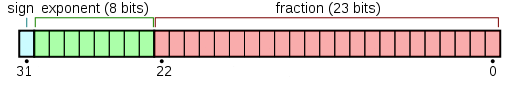
\includegraphics[scale=0.8]{foto/float.png}
\caption{Suddivisione della stringa binaria \textit{float} \cite{ref:float}}
\end{figure}
\ \\ \newline
Primo passaggio per il calcolo del valore rappresentato è la sottrazione del bias all'esponente.
\newline
Immettendo i dati nella formula \eqref{eq:bias}, otteniamo il seguente risultato:
\ \\
\begin{equation}
    bias_{float} = 2^{8-1}-1 = 2^{7}-1 = 128-1 = 127
\end{equation}
\begin{equation}
   esponente = \sum_{i=0}^{7} bit_{23+i}*2^{i} - bias_{float}
\end{equation}
\ \\
\newline
Passaggio successivo è la conversione della mantissa, che avviene secondo l'usuale metodo di conversione binaria, con la sola differenza che gli esponenti sono negativi:
\ \\
\begin{equation}
    mantissa = 1 + \sum_{i=1}^{23} bit_{23-i}*2^{-i} 
\end{equation}
\ \\
\newline
Ora che tutte le informazioni sono pronte, è possibile modificare la formula \eqref{eq:conversione_scientifica} ottenendo la seguente espressione finale:
\begin{equation}
    \begin{aligned}
        numero &= (-1)^{segno} * mantissa * 2^{esponente} \\
        &= (-1)^{segno} *( 1 + \sum_{i=1}^{23} bit_{23-i}*2^{-i}) * (\sum_{i=0}^{7} bit_{23+i}*2^{i} - bias_{float})
    \end{aligned}
\end{equation}








\newpage
Il tipo \textit{double} a doppia precisione è costituito, invece, da 64 bit:
\begin{itemize}
    \item 1 bit per il segno (0 se positivo, 1 altrimenti)
    \item 11 bit per l'esponente
    \item 52 bit per la mantissa
\end{itemize}
\ \\
Supponendo sempre la rappresentazione in big-endian (bit più significativo a sinistra), la nuova sequenza può essere suddivisa come segue:
\newline
\begin{figure}[h]
\centering
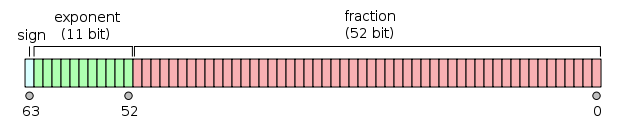
\includegraphics[scale=0.6]{foto/double.png}
\caption{Suddivisione della stringa binaria \textit{double} \cite{ref:double}}
\end{figure}
\ \\ \newline
I passaggi per il calcolo del valore numerico effettivo sono completamente analoghi a quelli citati per la singola precisione.
\newline \newline
Il bias è ricavato dalla formula \eqref{eq:bias}, ottenendo il seguente risultato:
\ \\
\begin{equation}
    bias_{double} = 2^{11-1}-1 = 2^{10}-1 = 1024-1 = 1023
\end{equation}
\begin{equation}
   esponente = \sum_{i=0}^{10} bit_{52+i}*2^{i} - bias_{double}
\end{equation}
\ \\
\newline
La mantissa è ottenuta tramite conversione binaria, ricordando però l'importanza dell'uso di esponenti negativi:
\ \\
\begin{equation}
    mantissa = 1 + \sum_{i=1}^{52} bit_{52-i}*2^{-i} 
\end{equation}
\ \\
\newline
Modificando infine la formula \eqref{eq:conversione_scientifica} come citato poco prima, si ottiene la seguente espressione finale:
\begin{equation}
    \begin{aligned}
        numero &= (-1)^{segno} * mantissa * 2^{esponente} \\
        &= (-1)^{segno} *( 1 + \sum_{i=1}^{52} bit_{52-i}*2^{-i}) * (\sum_{i=0}^{10} bit_{52+i}*2^{i} - bias_{double})
    \end{aligned}
\end{equation}



\newpage
I metodi di rappresentazione sopracitati consentono di esprimere un range di numeri reali molto ampio, però esistono delle particolari classi di numeri che costituiscono un limite computazionale per la CPU.
\newline \newline
Queste classi si dividono in:
\begin{itemize}
    \item zeri con segno
    \item infiniti con segno
    \item numeri \textit{normalizzati} finiti
    \item numeri \textit{denormalizzati} finiti
    \item NaN (Not a Number)
    \item numeri indefiniti
\end{itemize}
\ \\
Gli \textit{zeri con segno} sono delle particolari rappresentazioni del valore zero, aventi lo stesso valore nelle operazioni matematiche, ma che possono essere utili per indicare la direzione da cui avviene un underflow numerico.
\newline \newline
Gli \textit{infiniti con segno} rappresentano, rispettivamente, il più grande valore positivo e negativo che si può esprimere in floating-point.
\newline
A differenza degli zeri, il segno degli infiniti viene sempre considerato ed è possibile eseguire operazioni aritmetiche tra infiniti in modo corretto.
\newline
Possono anche essere utilizzati per rappresentare un overflow numerico.
\newline \newline
Qualsiasi numero finito compreso tra 0 (escluso) e $\pm \infty$ che può essere rappresentato in virgola mobile secondo le modalità citate precedentemente, viene anche detto numero \textit{normalizzato}.
\newline
Quando però questi numeri tendono infinitesimamente a zero, il valore massimo assunto dall'esponente della rappresentazione usata potrebbe non essere sufficiente per quantificare il numero effettivo di zeri dopo la virgola che precedono la prima cifra significativa, ed in questo caso si parla di numeri \textit{denormalizzati}.
\newline
La denormalizzazione di un numero avviene tramite graduali underflow, cioè supponendo di inserire un certo numero di zeri maggiormente significativi (shift a destra) fino a quando il valore non rientra nel range rappresentabile ed eliminando quindi alcune delle informazioni che costituiscono il numero effettivo, con conseguente perdita di precisione.
\newline
In casi particolari, potrebbe anche capitare che vengano scartati tutti i bit che costituivano il numero, con il risultato che quando si rientra nel range rappresentabile il valore ottenuto è zero.
\newline \newline
I \textit{NaN}, come suggerisce il nome, non sono numeri e pertanto non appartengono alla retta dei reali rappresentabili secondo la notazione normalizzata.
\newline
In questa categoria rientrano tutti quei numeri che hanno il massimo esponente possibile ed una mantissa non nulla, il bit del segno non viene invece considerato. 
\newline
Non hanno un effettivo utilizzo in termini matematici, ma consentono di segnalare eccezioni durante l'esecuzione di operazioni floating-point.




\newpage
Ultimo componente fondamentale della CPU nella gestione delle operazioni x86 è il registro EFLAGS a 32 bit, contenente i bit di \textit{status}, di \textit{controllo} e di \textit{sistema}.
\begin{figure}[h]
\centering
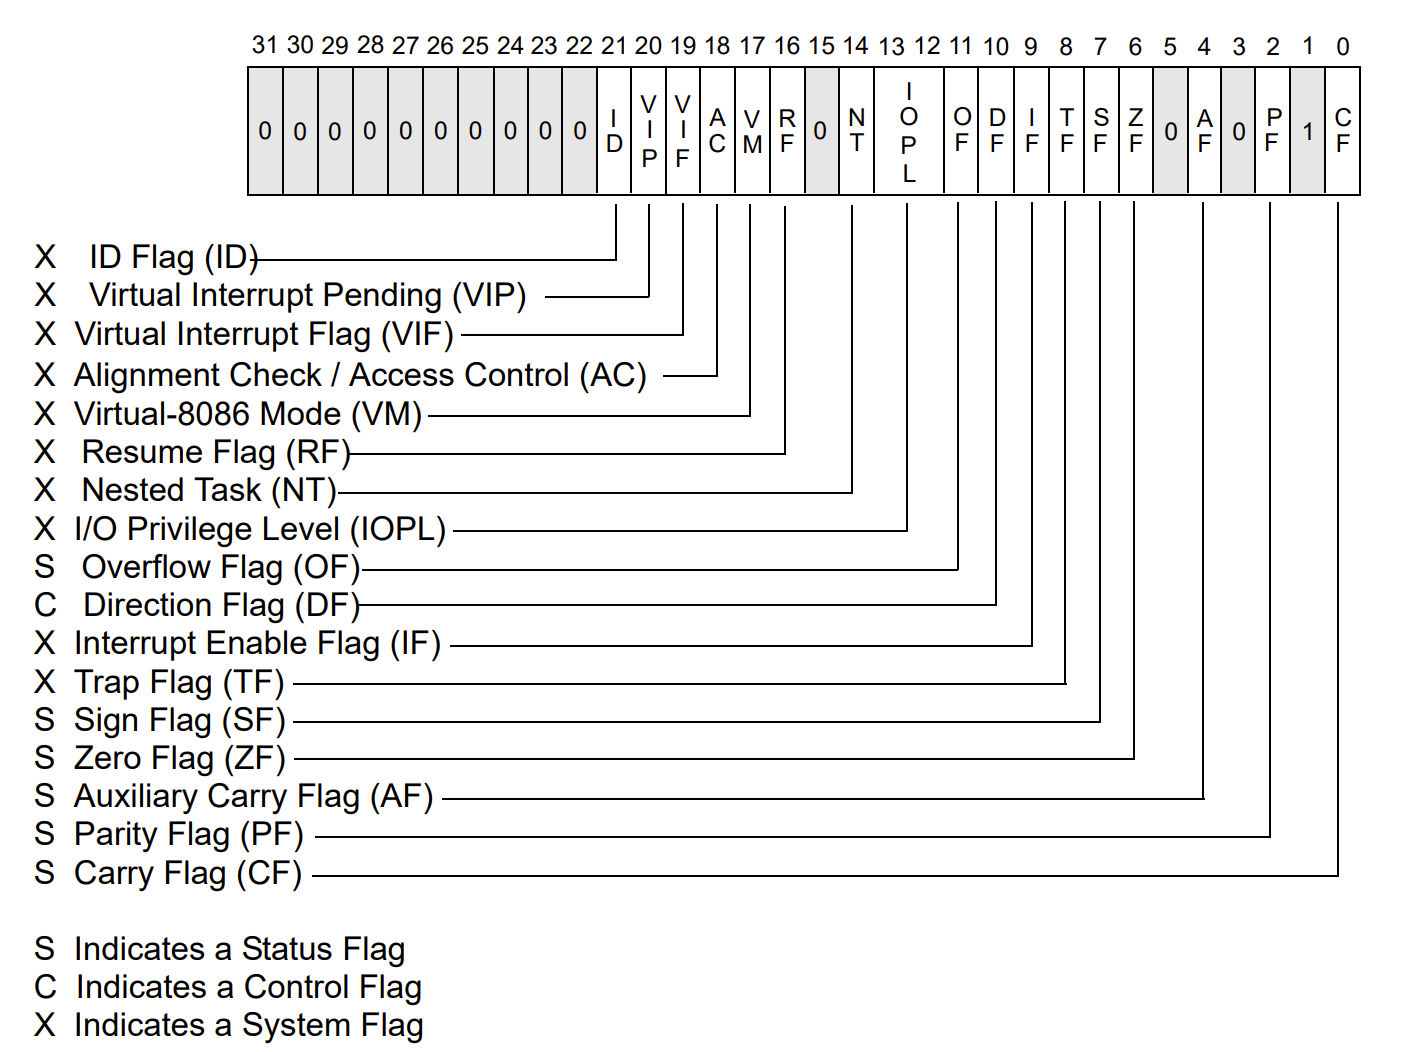
\includegraphics[width=0.786\linewidth]{foto/registro_eflags.png}
\caption{Struttura interna del registro EFLAGS \cite{ref:manuale_intel_1}}
\label{fig:registro_eflags}
\end{figure}
\newline
Ogni volta che viene eseguita un'istruzione aritmetica, i bit che costituiscono il gruppo di \textit{status} subiscono delle modifiche e questi saranno poi utilizzati, ad esempio, da operazioni di controllo come il costrutto \textit{if-else} per decidere se una condizione sia vera o falsa.
\newline
Ne segue quindi che la simbolizzazione di questi bit consente di dividere lo studio dell'esecuzione in due universi paralleli, uno in cui la condizione è verificata ed un altro in cui non lo è, e per questo motivo nella tesi ci si è concentrati sui bit riportati di seguito.
\newline \newline
Il \textit{Carry Flag} (CF, bit 0) viene settato se è stato generato del riporto da parte del bit più significativo del risultato, segnalando quindi un possibile overflow nell'operazione effettuata.
\newline \newline
Il \textit{Parity Flag} (PF, bit 2) viene settato se il byte meno significativo del risultato ha i bit settati ad 1 in numero pari.
\newline \newline
L' \textit{Auxiliary Carry Flag} (AF, bit 4) viene settato se è stato generato del riporto da parte di uno (o più) dei 4 bit meno significativi del risultato.
\newline \newline
Il \textit{Zero Flag} (ZF, bit 6) viene settato se il risultato dell'operazione è 0.
\newline \newline
Il \textit{Sign Flag} (SF, bit 7) viene utilizzato solo se gli operandi sono con segno ed assume il valore del bit più significativo del risultato, ovvero 0 se è positivo o 1 altrimenti.
\newline \newline
L' \textit{Overflow Flag} (OF, bit 11) viene settato in caso di overflow o underflow, rispettivamente se il risultato è troppo grande oppure troppo piccolo per essere rappresentato nel formato di destinazione.





\newpage
\section{Floating-Point in x87 e la FPU}
La famiglia di istruzioni x87 è un subset aggiuntivo di x86, definisce la rappresentazione dei numeri a doppia precisione estesa nel tipo \textit{long double} e viene gestita da un nuovo componente nel processore chiamato Floating Point Unit (FPU).
\newline \newline
Occorre notare innanzitutto che il nome \textit{long double} assegnato a questa nuova rappresentazione è specifico del linguaggio utilizzato in questa tesi, mentre altri linguaggi potrebbero utilizzare una nomenclatura diversa.
\newline
Inoltre, il compilatore C non associa esplicitamente la doppia precisione estesa a questo tipo a meno che non venga specificato il flag di compilazione \textit{"-mfpmath=387"}.
\newline \newline
L'esecuzione delle istruzioni x87 avviene nella FPU, dotata di un proprio ambiente completamente separato dal resto della macchina, ed al cui interno sono presenti:
\begin{itemize}
    \item 8 registri dati da 80 bit chiamati ST(i), con $i = 0,1,...,7$
    \item 3 registri di controllo da 16 bit (status, control e tag)
    \item puntatore all'ultima istruzione eseguita
    \item puntatore all'ultimo dato
    \item registro degli opcode
\end{itemize}
\ \\
Una particolarità nel funzionamento della FPU è la sua gestione a \textbf{stack} dei dati.
\newline
I registri dati non sono delle locazioni di memoria speciali, bensì sono organizzati in uno stack crescente verso il basso dove il registro in cima è sempre referenziabile tramite un puntatore chiamato TOP (\textit{top of stack}).
\newline \newline
L'operazione di memorizzazione di un nuovo valore nei registri avviene tramite una \textit{push} del registro che conterrà il valore, il quale diventerà la nuova cima dello stack e sarà referenziato da TOP.
\newline
In modo analogo, l'operazione di estrazione di un valore avviene tramite una \textit{pop} del registro puntato da TOP, il quale andrà poi a puntare alla nuova cima dello stack. 
\newline \newline
Lo stato di esecuzione della FPU è descritto all'interno del registro \textit{status}, il quale contiene informazioni sulle eccezioni delle operazioni, sul puntatore alla cima dello stack e sui \textit{condition code}.
\newline
Questi ultimi sono 4 bit che hanno uno scopo molto simile ai bit studiati nel registro EFLAGS, e vengono settati nelle operazioni aritmetiche o di confronto tra floating-point.
\newline
Se presi i bit che costituiscono il registro e raggruppati in una singola sequenza, questa viene anche detta \textit{FPU Status Word}.
\newline \newline
Il registro \textit{control} contiene informazioni sulla precisione dei calcoli e sulla \textbf{rounding mode} applicata, dove quest'ultima è documentata più avanti.
\newline
La sequenza di bit viene detta \textit{FPU Control Word}.
\newline \newline
Infine, il registro \textit{tag} indica il contenuto dei registri dati, assegnando ad ognuno di essi un particolare codice a seconda che il contenuto sia un numero speciale, zero oppure semplicemente vuoto.
\newline
La sequenza nel complesso viene anche detta \textit{FPU Tag Word}.





\newpage
Il tipo \textit{long double} a doppia precisione estesa è costituito da 80 bit:
\begin{itemize}
    \item 1 bit per il segno (0 se positivo, 1 altrimenti)
    \item 15 bit per l'esponente
    \item 1 bit speciale
    \item 63 bit per la mantissa
\end{itemize}
\ \\
Supponendo la rappresentazione in big-endian (bit più significativo a sinistra), la sequenza inserisce il bit speciale nel seguente modo:
\newline
\begin{figure}[h]
\centering
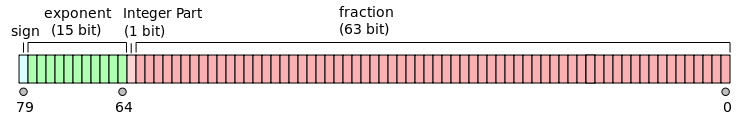
\includegraphics[scale=0.5]{foto/80_bit.png}
\caption{Suddivisione della stringa binaria \textit{double-extended} \cite{ref:80_bit}}
\end{figure}
\ \\ \newline
I passaggi per il calcolo del valore numerico effettivo rimangono inalterati rispetto a quelli mostrati per i tipi x86.
\newline \newline
Dalla formula \eqref{eq:bias} si calcola il bias, ottenendo il seguente risultato:
\ \\
\begin{equation}
    bias_{long\_double} = 2^{15-1}-1 = 2^{14}-1 = 16384-1 = 16383
\end{equation}
\begin{equation}
   esponente = \sum_{i=0}^{14} bit_{64+i}*2^{i} - bias_{long\_double}
\end{equation}
\ \\
\newline
La mantissa viene calcolata sempre con la conversione binaria, ricordando gli esponenti negativi:
\ \\
\begin{equation}
    mantissa = 1 + \sum_{i=1}^{63} bit_{63-i}*2^{-i} 
\end{equation}
\ \\
\newline \newline
In forma generale, è possibile applicare la formula \eqref{eq:conversione_scientifica} modificata per il calcolo del valore numerico, ma il bit speciale gioca un ruolo fondamentale nell'effettivo significato assunto dal numero.
\newline \newline
In questa tesi non saranno riportate tutte le casistiche particolari e le possibili combinazioni di valori che definiscono i numeri speciali, in quanto implementare le operazioni x87 all'interno di SymQEMU non è stato oggetto di studio, ma ci si è concentrati solo sulla parte 32/64 bit. Il resto sarà lasciato come lavoro futuro.




\newpage
\section{Rounding Mode}
Quando avviene una qualsiasi operazione floating-point, il processore cerca sempre di fornire come risultato un numero reale infinitesimamente preciso, ma il massimo numero di bit che ogni rappresentazione mette a disposizione limita la precisione del calcolo e pertanto vengono eseguiti degli arrotondamenti.
\newline \newline
All'interno della CPU, e più specificatamente nella FPU, sono presenti 2 bit di controllo che prendono il nome di \textit{Rounding Control Field} (RC Field) e che impostano la \textbf{rounding mode} da applicare al momento del calcolo.
\newline \newline
Queste si dividono fondamentalmente in due categorie:
\begin{itemize}
    \item arrotondamento diretto ad un intero
    \item arrotondamento all'intero più vicino
\end{itemize}
\ \\
\newline
La politica \textit{Rounding down} arrotonda direttamente al più grande numero esatto inferiore all'approssimazione ottenuta, ovvero effettua un arrotondamento per difetto, applicando la seguente formula:
\begin{equation}
    y = floor(x) = \lfloor x \rfloor
\end{equation}
\ \\
\newline
La politica \textit{Rounding up} arrotonda direttamente al più grande numero esatto superiore all'approssimazione ottenuta, e può essere vista come un arrotondamento per eccesso facente uso della seguente formula:
\begin{equation}
    y = ceil(x) = \lceil x \rceil
\end{equation}
\ \\
\newline
La politica \textit{Rounding towards zero} arrotonda direttamente alla parte intera del risultato, quindi troncando completamente la parte decimale, ed applicando un arrotondamento per eccesso o difetto a seconda del segno del numero:
\begin{equation}
    \begin{aligned}
        y &= sign(x) * \lfloor |x| \rfloor \\
        &= \begin{cases} \lceil x \rceil, \  x < 0 \\ \lfloor x \rfloor, \  x \geq 0 \end{cases}
    \end{aligned}
\end{equation}
\ \\
\newline
La politica \textit{Rounding away from zero} è analoga a quella \textit{towards zero}, con la sola differenza che l'arrotondamento per eccesso o difetto a seconda dei segni avviene in modo opposto alla precedente:
\begin{equation}
    \begin{aligned}
        y &= sign(x) * \lceil |x| \rceil \\
        &= \begin{cases} \lceil x \rceil, \  x \geq 0 \\ \lfloor x \rfloor, \  x < 0 \end{cases}
    \end{aligned}
\end{equation}



\newpage
La politica \textit{Rounding half away from zero} si applica solo nel caso di numeri aventi parte decimale pari a 0.5 e, a seconda del segno, l'arrotondamento viene fatto all'intero più grande subito successivo:
\begin{equation}
    y = ceil(x) = sign(x) * \lfloor |x|+0.5 \rfloor
\end{equation}
\ \\
\newline
Infine, la politica \textit{Rounding half to even} viene anch'essa applicata solo nel caso di numeri con parte decimale uguale a 0.5, però l'arrotondamento può essere fatto sia all'intero subito dopo che a quello subito prima.
\newline
Quest'ultima è la modalità di default utilizzata per tutte le operazioni in virgola mobile ed è impostata dall'OS al suo avvio.
\newline \newline \newline
Durante lo sviluppo di un progetto la scelta della rounding mode applicata risulta quindi essere un'informazione fondamentale, dato che la perdita di precisione nel corso dei calcoli potrebbe diventare non indifferente, e pertanto occorre studiare ogni situazione e scegliere quella più adatta alle proprie necessità.
\newline \newline
In questo progetto, per questioni di maggiore semplicità nel calcolo della soddisfacibilità delle formule e nella generazione dei nuovi input, si è deciso di lasciare la modalità di arrotondamento di default (\textit{rounding half to even}). 
\newline
Il supporto ad altre modalità di arrotondamento potrà essere aggiunto come contributo futuro.








\newpage
\section{Operazioni SSE e registri XMM}
L'architettura x86 (e x86\_64) studiata in questa tesi si avvale della modalità di esecuzione multiprocesso detta \textit{SIMD} (Single Instruction Multiple Data), la quale ha introdotto la tecnologia MMX ed i set di istruzioni SSE/SSE2.
\newline \newline
La politica \textit{SIMD} consente al processore di suddividere un registro in parti uguali, di dimensione in bit minore rispetto al numero iniziale, ed immagazzinare al suo interno molteplici piccoli dati piuttosto che un singolo dato che occupi l'intero spazio disponibile.
\newline
Questi gruppi di dati raccolti all'interno di un unico registro vengono detti \textit{packed data}, e su di essi è possibile applicare istruzioni che effettuino parallelamente una stessa operazione su ogni singolo componente del gruppo.
\newline \newline
Quando questa tecnologia venne inizialmente introdotta era possibile "impacchettare" solo valori binari, in tempi più moderni è stata estesa anche ad alcune strutture dati come array e struct.
\newline \newline
La tecnologia \textit{MMX} introduce due nuove tipologie di registri:
\begin{itemize}
    \item MMX: 8 registri a 64 bit, supportano esclusivamente \textit{packed integer}
    \item XMM: 8 registri a 128 bit, supportano \textit{packed integer} e \textit{packed floating-point}
\end{itemize}
Vengono anche definite le prime istruzioni che effettuano operazioni parallele, inizialmente però solo sui registri MMX e quindi operazioni intere.
\newline \newline
Il set di istruzioni \textit{SSE} introduce il supporto alle operazioni parallele su \textit{packed floating-point} tramite i registri XMM, però i dati dovevano essere necessariamente a singola precisione.
\newline
Inoltre, estende le operazioni su \textit{packed integer} per i registri MMX.
\newline \newline
Il set di istruzioni \textit{SSE2} consente di effettuare operazioni parallele su \textit{packed floating-point} a doppia precisione ed estende le operazioni introdotte da SSE anche ai registri XMM.
\newline \newline
\begin{figure}[h]
\centering
\begin{subfigure}{.5\textwidth}
  \centering
  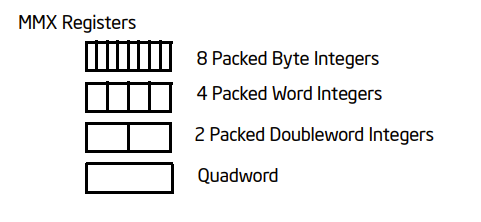
\includegraphics[width=1\linewidth]{foto/mmx.png}
  \label{fig:sub1}
\end{subfigure}%
\begin{subfigure}{.5\textwidth}
  \centering
  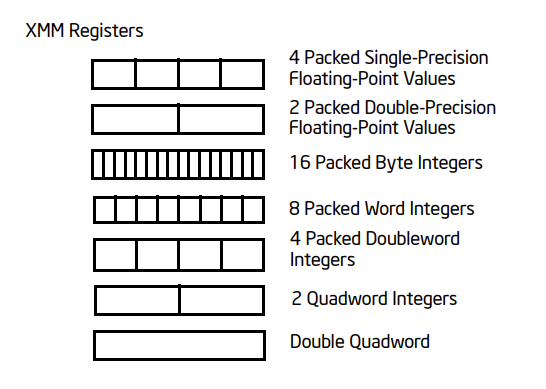
\includegraphics[width=1.005\linewidth]{foto/xmm.png}
  \label{fig:sub2}
\end{subfigure}
\caption{Possibile suddivisione dei nuovi registri MMX e XMM dopo SSE2}
\label{fig:mmx}
\end{figure}



\newpage
Un esempio di istruzione di questo tipo è la PADD (\textit{Packed Add Integers}), che consente di applicare l'operazione di somma a molteplici blocchi di una stringa.
\newline
Graficamente, questa istruzione può essere rappresentata nel seguente modo:
\begin{figure}[h]
    \centering
    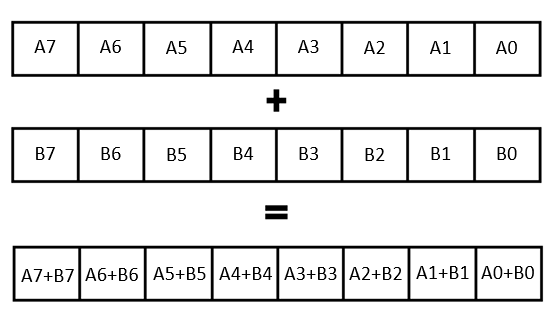
\includegraphics[width=0.75\linewidth]{foto/packed_add.png}
    \captionsetup{format=hang}
    \caption{Operazioni effettuate dalla PADDB, supponendo stringhe da 64 bit}
    \label{fig:padd}
\end{figure}
\ \\ \newline
Poiché l'istruzione PADDB opera sui byte, la stringa viene prima suddivisa in 8 blocchi di 8 bit ciascuno, quindi viene fatta la somma tra i rispettivi blocchi nella destinazione.
\newline
È possibile applicare operazioni packed anche sui floating-point, ad esempio tramite l'istruzione ADDPS (\textit{Add Packed Single-Precision Floating-Point Values}).
\newline \newline \newline
Per raggiungere l'obiettivo di questa tesi ci si è concentrati sui set di istruzioni SSE/SSE2, andando ad operare simbolicamente sul contenuto dei registri XMM.





\chapter{Implementazione}
\ \\
\section{Obiettivo}
L'obiettivo di questa tesi è sviluppare un primo prototipo di supporto alle operazioni floating-point all'interno dell'esecutore concolico SymQEMU, nello specifico iniziando dalle operazioni matematiche di somma, differenza, prodotto e divisione.
\newline \newline
Per fare ciò è stato fatto un ampio studio dell'attuale codice di SymQEMU, precisamente nelle seguenti sezioni:
\begin{itemize}
    \item runtime simbolico di SymQEMU, che si occupa dell'invocazione dei metodi per la costruzione delle formule
    \item runtime simbolici di SymCC e QSYM, che si occupano dell'effettiva costruzione simbolica delle formule
    \item comunicazione tra i runtime di SymQEMU e SymCC/QSYM
    \item traduzione delle espressioni simboliche generate in espressioni risolvibili dal solver Z3 e la loro risoluzione
\end{itemize}
\ \\
Nei paragrafi successivi saranno analizzate nello specifico le modifiche apportate, di cui un breve riassunto del lavoro svolto è riportato di seguito.
\newline \newline
Innanzitutto è stato necessario decidere quali nuove operazioni implementare simbolicamente, identificare gli opcode ad esse associate e studiare questi ultimi tramite il manuale Intel per comprenderne appieno il funzionamento.
\newline
Per fare ciò sono stati creati molteplici codici di test, contenenti le operazioni in questione, e analizzati i disassemblati sotto diversi flag di compilazione per capire il comportamento adottato dal compilatore e gli opcode assegnati.
\newline
È importante precisare che in questo studio si è fatto uso del compilatore \textit{gcc}, pertanto i collegamenti tra operazione ed opcode mostrati in seguito potrebbero non rimanere consistenti se utilizzati compilatori diversi.
\newline \newline
Successivamente sono stati fatti degli esercizi per apprendere l'utilizzo dell'SMT solver Z3, basandosi su esempi forniti dagli sviluppatori, al fine di prendere confidenza con i metodi per la costruzione delle espressioni simboliche e comprendere il flusso risolutivo.
\newline \newline
Infine, dopo aver compreso il flusso esecutivo compiuto dalle operazioni simboliche all'interno di SymQEMU, si è passati ad agire sulle singole sezioni precedentemente indicate al fine di inserire il riconoscimento delle nuove istruzioni e la definizione delle funzioni necessarie a rappresentarle simbolicamente.







\newpage
\section{Perché agire solo sulla famiglia SSE/SSE2}
La prima parte del lavoro, come accennato in precedenza, si è incentrata sull'analisi del compilatore \textit{gcc} tramite un ampio spettro di test.
\newline \newline
Dato uno stesso codice di partenza, diversi compilatori possono emettere istruzioni diverse per via delle scelte progettuali compiute durante la loro realizzazione: alcuni potrebbero prediligere certi opcode per una maggiore efficienza, altri applicare diverse tecniche di ottimizzazione del codice, altri ancora fare uso di componenti della CPU in modo automatico rispetto a compilatori in cui sarebbe invece necessaria un'indicazione esplicita tramite flag.
\newline \newline
Per studiare quindi il comportamento adottato dal nostro compilatore, si sono eseguiti i seguenti test sotto diversi livelli di ottimizzazione e flag di compilazione:
\begin{itemize}
    \item confronto ordered
    \item confronto unordered
    \item conversione da intero a floating-point
    \item conversione da floating-point a intero
    \item somma intera e floating-point
    \item differenza intera e floating-point
    \item prodotto intero e floating-point
    \item divisione intera e floating-point
\end{itemize}
\ \\
Come si può notare, i test sono stati incentrati principalmente sulle operazioni più semplici e basilari, così da rimanere in una astrazione simbolica relativamente intuitiva e priva di costrutti complessi.
\newline
Contemporaneamente all'analisi dei disassemblati, è anche stato analizzato l'esecutore simbolico, identificando quali operazioni tra quelle di nostro interesse fossero già implementate e gestite simbolicamente e quali invece venissero trattate solo concretamente. 
\newline \newline
In merito alle operazioni aritmetiche intere, nel nostro caso gestite dalle più comuni ADD, SUB, MUL e DIV, SymQEMU implementava già il supporto simbolico.
\newline
Per tutte le operazioni che invece comprendevano almeno uno dei parametri in virgola mobile, sia aritmetiche che di conversione, vi era soltanto la gestione concreta ma non quella simbolica.
\newline \newline
Per questo motivo, al fine di poter effettuare l'analisi completa di un semplice programma, si è deciso inizialmente di implementare simbolicamente la somma, conversione e confronto ordered per floating-point.
\newline
È importante sottolineare che il set di istruzioni SSE mette a disposizione due opcode diversi a seconda che gli operandi siano in singola o doppia precisione, tralasciando per il momento la doppia precisione estesa perché gestita da istruzioni specifiche per la FPU.
\newline
Ai fini di questo studio l'implementazione è stata effettuata relativamente alle operazioni in singola precisione, lasciando la doppia precisione come lavoro futuro.




\newpage
Durante l'analisi dei test precedentemente elencati sono venute alla luce delle particolarità sul comportamento del compilatore, che verranno successivamente illustrate, ma facendo prima una breve introduzione sui livelli di ottimizzazione del codice messi a disposizione al fine di comprendere meglio quanto verrà mostrato in seguito.
\newline \newline
Il compilatore \textit{gcc} mette a disposizione diversi livelli di ottimizzazione, di cui i tre più utilizzati sono impostabili tramite i flag "\textit{-O1/2/3}":
\begin{itemize}
    \item il livello 1 riduce la lunghezza del codice ed il tempo richiesto per l'esecuzione, aumentando invece tempo di compilazione ed uso della memoria
    \item il livello 2 aumenta notevolmente le performance del codice, generalmente introducendo nuovi set di istruzioni (es. AVX ed operazioni parallele), ma incrementando ulteriormente il tempo di compilazione
    \item il livello 3 non differisce molto in termini di ottimizzazione dal livello 2, sostanzialmente vengono vettorizzati i loop e rese più efficienti le subroutine
\end{itemize}
\ \\
I programmi compilati con ottimizzazione nulla o di livello 1 riportavano gli opcode più basilari, con la differenza che in quelli ottimizzati era spesso presente \textit{inline} di funzioni, pertanto tutte le istruzioni incontrate sono state riportate in una tabella e studiato il loro significato tramite manuale.
\newline \newline
Il secondo livello di ottimizzazione si è rivelato essere il più interessante, in particolare nei test facenti uso della doppia precisione estesa.
\newline
Come accennato nel capitolo precedente, l'uso del tipo \textit{long double} ad 80 bit dovrebbe essere lasciato alla FPU ed al set di istruzioni x87, mentre il compilatore si limitava all'utilizzo delle istruzioni SSE per floating-point.
\newline
Approfondendo questo particolare comportamento, si è scoperto che il compilatore non fa uso della FPU e del suo set di istruzioni se non specificato tramite flag, inoltre il tipo \textit{long double} non viene effettivamente interpretato come precisione ad 80 bit ma come semplice doppia precisione.
\newline
Facendo invece uso del flag "\textit{-mfpmath=387}", viene forzato l'uso della FPU in qualsiasi operazione floating-point a prescindere dalla precisione richiesta, pertanto si è concluso che per questo studio sarebbe stato sufficiente implementare le operazioni da noi scelte limitandosi all'uso delle istruzioni SSE/SSE2.
\newline \newline
Infine, il terzo livello di ottimizzazione non ha introdotto significative differenze rispetto al precedente, pertanto ha avuto un contributo trascurabile nell'analisi.
\newline \newline





\newpage
\section{Architettura di SymQEMU, SymCC, QEMU e QSYM}
L'esecutore concolico \textit{SymQEMU} si basa su diversi framework già esistenti, prendendone i punti di forza e creando un esecutore flessibile e performante allo stesso tempo, per l'esecuzione simbolica su codice binario.
\newline \newline
Il suo flusso esecutivo può essere riassunto nel seguente modo:
\begin{enumerate}
    \item traduzione delle istruzioni del file eseguibile in un linguaggio intermedio
    \item aggiunta delle istruzioni per la rappresentazione simbolica nel linguaggio intermedio
    \item traduzione del codice generato nel punto 2 in linguaggio macchina per l'architettura sottostante
\end{enumerate}
\ \\
Utilizzando l'approccio alla compilazione ispirato da \textit{QSYM}, viene lasciato alla CPU il compito di eseguire tutte le operazioni concrete e simboliche del codice tradotte, ottenendo una velocità esecutiva notevole.
\newline
Questa scelta è stata fatta in contrapposizione ad un'altra tecnica molto usata, ovvero quella dell'\textit{interpretazione} del codice, che favorisce una più complessa analisi istruzione per istruzione al costo delle prestazioni.
\newline \newline
Il primo framework su cui si basa SymQEMU è \textit{SymCC}, un esecutore simbolico compilation-based per file sorgenti, che fa uso di un linguaggio macchina intermedio chiamato LLVM per inserire le funzioni che definiscono le espressioni simboliche.
\newline
Il nuovo codice ottenuto è poi tradotto in linguaggio macchina, ottenendo così un eseguibile finale che potrà essere testato un numero indefinito di volte su input diversi senza la necessità di interpretare simbolicamente ogni volta le medesime istruzioni.
\newline \newline
Riportiamo graficamente il flusso esecutivo compiuto da SymCC:
\begin{figure}[h]
    \centering
    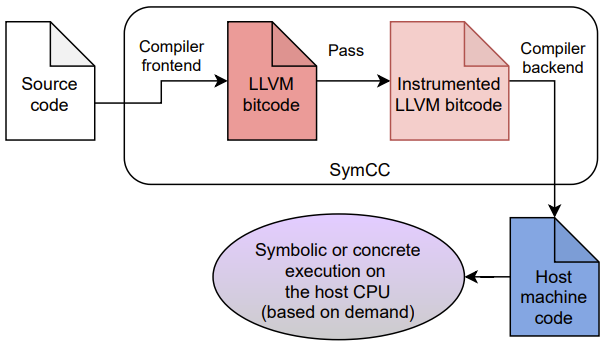
\includegraphics[width=0.59\linewidth]{foto/flusso_symcc.png}
    \caption{SymCC: partendo dal codice sorgente, viene effettuata la traduzione in codice} {LLVM e sono aggiunte le funzioni simboliche, infine si traduce il tutto nuovamente} {in un linguaggio comprensibile dall'architettura sottostante                                 }    \label{fig:flusso_symcc}
\end{figure}
\ \\ \newline
Al suo interno SymCC mette a disposizione due backend per la costruzione e risoluzione delle formule, uno utilizzabile principalmente per scopi di debug ed uno basato su \textit{QSYM}. In questa tesi ci siamo concentrati sul secondo runtime, in quanto è quello utilizzato da SymQEMU.



\newpage
SymQEMU fa uso una strategia di analisi molto simile a questa di SymCC, con la differenza che analizza il codice binario anziché sorgente come base da cui partire per effettuare la traduzione in linguaggio intermedio.
\newline\newline
Il secondo framework utilizzato da SymQEMU è \textit{QEMU}, un noto programma per la virtualizzazione di interi sistemi operativi e l'emulazione dell'architettura di molti processori.
\newline
Nel nostro caso si è fatto riferimento alla famiglia di processori x86 e x86\_64.
\newline \newline
In particolare, viene esteso un componente di QEMU chiamato \textit{Tiny Code Generator}: quando utilizzato per l'emulazione di architetture, QEMU traduce il codice scritto nell'architettura della macchina host in un linguaggio intermedio, chiamato appunto TCG, e che sua volta sarà poi tradotto in linguaggio macchina comprensibile per la nuova architettura che si sta testando.
\newline
Queste operazioni TCG sono proprio quelle che dovranno essere eseguite dalla CPU emulata, sono scritte in questo linguaggio intermedio e poi convertite nelle corrispondenti istruzioni macchina seguendo specifici file di traduzione creati appositamente per ogni architettura.
\newline \newline
Così facendo l'esecutore simbolico rimane indipendente dall'architettura, ed un singolo blocco TCG è possibile eseguirlo su diversi sistemi facendo affidamento sul traduttore al linguaggio macchina sottostante.
\newline \newline
L'aggiunta però di una fase di traduzione intermedia ha costi sulle prestazioni non indifferenti, poiché l'operazione di disassembly su binari eseguibili  costituisce comunque un overhead inevitabile.
\newline \newline
Riassumendo, il flusso esecutivo di QEMU è il seguente:
\newline
\begin{figure}[h]
    \centering
    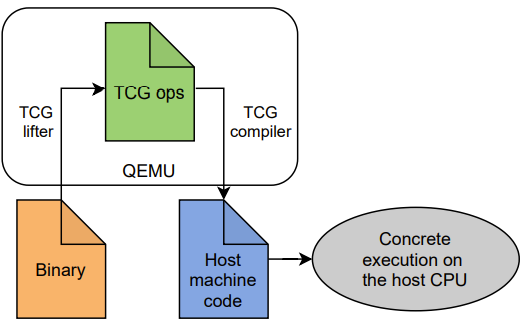
\includegraphics[width=0.625\linewidth]{foto/flusso_qemu.png}
    \caption{QEMU: il codice binario viene tradotto prima in TCG, dove vengono aggiunte} {le operazioni necessarie per la rappresentazione come espressioni simboliche, quindi} {il tutto viene riportato in codice macchina per essere eseguito concretamente sulla CPU simulata                                                                                                 }
    \label{fig:flusso_qemu}
\end{figure}
\newline \newline
L'intervento compiuto da SymQEMU è stato quello di ampliare le operazioni TCG messe a disposizione, inserendo nuovi costrutti che consentono di rappresentare simbolicamente un maggior numero di istruzioni macchina.




\newpage
Prima però di introdurre le modifiche da noi effettuate su SymQEMU, è opportuno spiegarne il flusso esecutivo analizzando i vari step in cui passa un singolo opcode.
\newline \newline
Si parta dal seguente frammento di codice, per semplicità facente uso della computazione intera:
\begin{figure}[h]
\begin{lstlisting}[xleftmargin=.35\textwidth,language=C]
int x = y + 42;
\end{lstlisting}
  \caption{Una semplice istruzione che somma 42 ad una variabile}
  \label{fig:tcg_1}
\end{figure}
\ \\
\newline
Compilando il codice con ottimizzazione si ottiene il seguente risultato:
\begin{figure}[h]
  \begin{lstlisting}[xleftmargin=.35\textwidth,language={[x86masm]Assembler}]
lea rsi,[rax+0x2a]
\end{lstlisting}
  \caption{L'istruzione \textit{lea} consente di caricare l'indirizzo e sommarvi la costante 42 (2A)}
  \label{fig:tcg_2}
\end{figure}
\ \\
\newline
Quando un generico binario viene lanciato da SymQEMU, il codice sorgente mostrato in Figura (\ref{fig:tcg_1}) non è noto, ma viene ricevuto in ingresso il contenuto di Figura (\ref{fig:tcg_2}).
\newline
Se elaborata tale istruzione, il suo corrispettivo TCG è il seguente:
\begin{figure}[h]
\begin{lstlisting}[xleftmargin=.33\textwidth,language=SymQEMU]
movi_i64 tmp12,$0x2a
add_i64 tmp2,rax,tmp12
ext32u_i64 rsi,tmp2
\end{lstlisting}
\caption{Il blocco risultante dall'operazione di traduzione in TCG}
\label{fig:tcg_3}
\end{figure}
\ \\
Le operazioni eseguite da questo blocco possono essere riassunte come uno spostamento di 64 bit, una somma di 64 bit ed infine un'estrazione di 32 bit.
\newline \newline
A prima vista si intuisce innanzitutto che QEMU opera esclusivamente a 64 bit, data la necessità di \textit{estrarre} un sottoinsieme del risultato nell'ultima operazione eseguita dal blocco.
\newline
Inoltre, la struttura prende direttamente spunto dalla sintassi AT\&T per x86.
\newline
La particolarità risiede nella presenza degli operandi $tmp$, che ci limiteremo a definire come dei registri aggiuntivi temporanei utilizzati per consentire l'esecuzione di passaggi intermedi.
\newline \newline \newline
Procediamo ora ad analizzare le singole istruzioni per comprendere meglio il funzionamento di TCG.
\newline \newline
La prima istruzione muove i 64 bit dell'operando 0x2A, che è un immediato data la presenza del simbolo \$ che lo precede, nel registro temporaneo tmp12.
\newline
Successivamente viene fatta una somma a 64 bit, dove i due addendi sono i registri rax e tmp12, mentre il risultato viene memorizzato in tmp2.
\newline
Infine, vengono estratti 32 bit unsigned dal registro tmp2 e memorizzati in rsi.




\newpage
Dopo l'aggiunta dello strato simbolico da parte di SymQEMU, il codice in Figura (\ref{fig:tcg_3}) assume la seguente forma:
\begin{figure}[h]
\begin{lstlisting}[language=SymQEMU, basicstyle=\small]
movi_i64 tmp12_expr,$0x0
movi_i64 tmp12,$0x2a

call sym_add_i64,$0x5,$1,tmp2_expr,rax,rax_expr,tmp12,tmp12_expr
add_i64 tmp2,rax,tmp12

movi_i64 tmp12,$0x4
call sym_zext,$0x5,$1,rsi_expr,tmp2_expr,tmp12
ext32u_i64 rsi,tmp2
\end{lstlisting}
\caption{Sono state aggiunte le istruzioni per la rappresentazione simbolica}
\label{fig:tcg_4}
\end{figure}
\ \\
Quello che si nota subito è la presenza di nuovi operandi, aventi il suffisso "expr", e di chiamate a funzioni con il prefisso "sym".
\newline \newline
Per facilità di comprensione il seguente blocco è stato suddiviso in tre parti, dove ognuna di esse rappresenta il risultato del processamento simbolico delle singole istruzioni, e sono analizzate di seguito.
\newline \newline
La prima istruzione incontrata era la MOV di un operando immediato.
\newline
Da un punto di vista simbolico, un operando immediato viene considerato come un input \textit{concreto} poiché conosciuto a tempo di compilazione, pertanto la regione di memoria dedicata alla rappresentazione simbolica del registro tmp12 viene inizializzata a 0.
\newline
Questa è una scelta progettuale di SymQEMU, dove inizializzare a 0 una regione di memoria simbolica significa che il registro associato ad essa contiene un valore concreto.
\newline
Dato che la variabile tmp12\_expr è stata definita concreta, è seguita semplicemente dall'esecuzione reale del codice iniziale.
\newline \newline
Successivamente, prima dell'esecuzione della add, è presente una chiamata alla funzione "sym\_add\_i64" seguita da una serie di parametri.
\newline
Questa funzione è esattamente una delle operazioni TCG introdotte da SymQEMU, in questo caso per rappresentare simbolicamente l'operazione di somma tra due interi a 64 bit, e mostra la strategia di SymQEMU di voler prima valutare l'espressione simbolica di un'operazione e poi eseguirla concretamente.
\newline
Il numero di parametri e l'analisi di questi verrà fatta più avanti, anche se ci limiteremo a dire che ogni funzione simbolica ha un numero variabile di parametri e accetta come operandi registri concreti, simbolici e lo stato della CPU simulata.
\newline \newline
Nell'ultimo blocco è inizialmente presente la MOV di un altro operando immediato nel registro tmp12, di cui notiamo l'assenza dell'inizializzazione a 0 della sua controparte simbolica perché già segnalata la sua concretezza all'inizio del codice.
\newline
Infine, la chiamata alla funzione "sym\_zext" è un'altra delle nuove operazioni definite e rappresenta la simbolizzazione dell'estrazione dei 32 bit unsigned compiuta al termine del blocco.





\newpage
È importante notare che nessuna di queste operazioni viene eseguita da SymQEMU, ma viene fatto affidamento sul sistema di traduzione fornito da QEMU per la conversione di quest'ultimo blocco in codice macchina per l'architettura interessata.
\newline
Dato però il suo utilizzo come emulatore di CPU, l'esecuzione delle funzioni può avvenire esclusivamente in user-mode, pertanto l'analisi simbolica non può essere effettuata su system-call perché entrerebbero altrimenti in kernel-mode.
\newline \newline \newline
L'ultimo framework utilizzato è \textit{QSYM}, da cui SymQEMU ha rielaborato i suoi metodi di gestione efficiente della memoria e la sua ottimizzazione nell'analisi delle espressioni: il primo consente di minimizzare lo spazio occupato dalle molteplici espressioni generate durante l'analisi, mentre il secondo riduce al minimo le operazioni ridondanti e cerca di sfruttare il più possibile i risultati già ottenuti per minimizzare i tempi.
\newline \newline
A livello di runtime, QSYM basa la sua analisi utilizzando una tecnica chiamata "\textit{Dynamic Binary Translation}" (DBT) dove, in contemporanea all'esecuzione del codice, sono inserite le istruzioni necessarie a rappresentare l'espressione simbolica.
\newline
Il risultato ottenuto è un nuovo blocco di codice, in cui sono state aggiunte le funzioni simboliche, che verrà poi analizzato per la costruzione dell'espressione finale e degli eventuali \textit{path constraints} andando ad eseguire solo le funzioni appena aggiunte.
\newline \newline
Per ottimizzare ulteriormente l'analisi, SymQEMU riprende anche un'altra strategia introdotta da QSYM chiamata \textit{block pruning}.
\newline
Viene costruito un call-stack nascosto (\textit{shadow call-stack}) che tiene conto delle espressioni più analizzate: così facendo, le valutazioni più frequenti possono essere effettuate in modo rapido ed efficiente perché già contenute in memoria, eliminando l'overhead dovuto alla ripetizione delle medesime operazioni.
\newline \newline \newline
In conclusione, raggruppando tutti i programmi appena citati, il flusso esecutivo di SymQEMU può essere riassunto nel seguente grafico:
\begin{figure}[h]
    \centering
    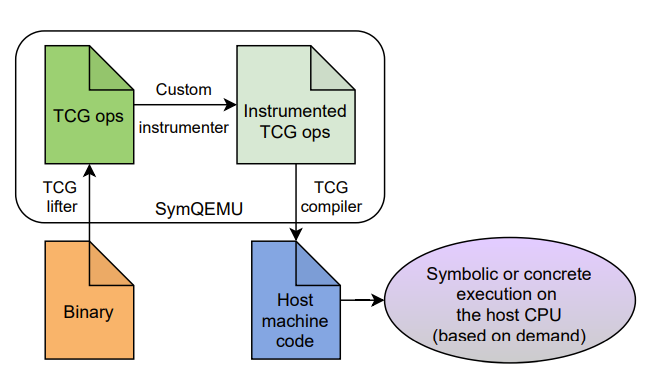
\includegraphics[width=0.7\linewidth]{foto/flusso_symqemu.png}
    \caption{Flusso complessivo di SymQEMU}
    \label{fig:flusso_symqemu}
\end{figure}
\ \\
Partendo quindi dal codice binario, QEMU traduce le istruzioni macchina in TCG, SymQEMU inserisce lo strato simbolico ed infine si ritorna a codice macchina per l'architettura sottostante.

\newpage
\section{Interventi in SymQEMU}
Primo passaggio per l'introduzione di una nuova funzione simbolica è partire da SymQEMU, andando ad operare nella catena di traduzione del codice binario in TCG, e definendo quello che sarà il corpo del gestore simbolico tramite le funzioni messe a disposizione da SymCC e QSYM.
\newline \newline
Abbiamo già detto che, affidandosi all'emulazione della CPU tramite QEMU, l'esecutore simbolico è in grado di tradurre del codice a basso livello in un linguaggio intermedio in cui è possibile introdurre le operazioni che costruiranno poi l'espressione simbolica finale.
\newline
All'interno dei file messi a disposizione da QEMU, infatti, ogni architettura ha un suo file specifico contenente tutto il flusso esecutivo che deve essere applicato affinché ogni istruzione possa essere tradotta correttamente, sia concretamente che simbolicamente, da parte della CPU simulata.
\newline \newline
Nel nostro caso si è andato a modificare il file di traduzione per l'architettura Intel x86 e x86\_64.
\newline \newline
Partendo quindi da un codice binario in ingresso, ogni singola istruzione macchina viene analizzata byte per byte dal file di traduzione più adatto, al cui interno sono definiti una serie di controlli che consentono di identificare le varie operazioni definite per una certa architettura.
\newline
Dopo aver caricato il primo byte dell'istruzione, nel caso dell'architettura Intel una delle prime operazioni eseguite è la verifica della presenza di prefissi speciali, ovvero byte che segnalino alla CPU di eseguire comportamenti particolari come, ad esempio, la ripetizione dell'operazione un certo numero di volte oppure l'accesso in memoria solo ad uno specifico segmento.
\newline
Nel caso in cui venga identificato un prefisso di questo tipo, vengono settati dei flag di cui occorrerà tenere conto nel corso dell'esecuzione concreta dell'istruzione, passando poi all'analisi del successivo byte nuovamente alla ricerca di un prefisso speciale.
\newline
Quando un certo byte supera tutti i controlli sopracitati senza attivarne alcuno, significa che quello attualmente analizzato è il primo byte effettivo rappresentante l'opcode da definire.
\newline \newline
Da qui inizia la determinazione dell'istruzione analizzata e dell'eventuale comportamento definito per essa.
\newline \newline
Tramite un unico costrutto "\textit{switch-case}" sul byte analizzato, facendo affidamento su delle euristiche definite dagli sviluppatori ed al byte stesso, si accede ad una tabella contenente le funzioni definite per la gestione delle istruzioni messe a disposizione dall'architettura x86.
\newline \newline
Per le operazioni floating-point però, poiché non ancora gestite simbolicamente, molte di queste funzioni non contenevano un vero e proprio corpo di operazioni da eseguire ma venivano lasciate al \textit{default} dello switch, il quale semplicemente mandava in esecuzione concreta l'istruzione stessa.
\newline
Esattamente questo è il punto in cui si è andati ad agire: prima dell'esecuzione concreta è stato inserito un controllo per assicurarsi che l'istruzione che stesse per essere eseguita fosse effettivamente quella desiderata e, in tal caso, invocata l'esecuzione del gestore simbolico da noi definito.



\newpage
La situazione iniziale da cui si è partiti a lavorare è la seguente:
\begin{figure}[h]
\begin{lstlisting}[xleftmargin=0\textwidth, language=SymQEMU]
0x40000011eb: f3 0f 58 c1   addss   %xmm1, %xmm0

---- 00000040000011eb 0000000000000000
movi_i64 tmp12,$0x318               pref=0xffff
add_i64 tmp8,env,tmp12              dead: 2  pref=0xf0b8
movi_i64 tmp12,$0x358               pref=0xffff
add_i64 tmp9,env,tmp12              dead: 1 2  pref=0xf078
call addss,$0x0,$0,env,tmp8,tmp9    dead: 0 1 2
\end{lstlisting}
    \caption{In alto l'input binario ricevuto da SymQEMU, sotto il TCG generato}
    \label{fig:addss_prima}
\end{figure}
\ \\
Per semplicità l'esempio mostrato fa riferimento alla prima operazione studiata in questo progetto, ovvero la somma tra due valori floating-point.
\newline
L'istruzione ADDSS (gestita in QEMU con la funzione addss) è una delle prime istruzioni floating-point implementate nell'architettura Intel x86, poiché appartenente alla famiglia SSE, ed effettua la somma tra due valori a singola precisione memorizzando il risultato nei 32 bit meno significativi del registro destinazione.
\newline \newline
Come possiamo vedere dalla Figura (\ref{fig:addss_prima}), a differenza di quanto mostrato invece in Figura (\ref{fig:tcg_4}), non vi è la presenza di alcuna chiamata ad una funzione del tipo "sym\_addss" prima dell'invocazione dell'esecuzione concreta dell'istruzione.
\newline
Questo perché, come appunto introdotto in precedenza, all'interno del file di traduzione di QEMU non è associata alcuna operazione simbolica al gestore della ADDSS, dal momento che si tratta di un'operazione floating-point.
\newline \newline
Per fare ciò bisogna definire un \textit{helper simbolico} all'interno del gestore, in modo tale che prima dell'esecuzione concreta dell'istruzione venga creata l'espressione simbolica della somma floating-point.
\newline
Un \textit{helper simbolico} è una funzione definita all'interno del runtime di SymQEMU che si occupa di gestire la memoria simbolica, quindi manipolando l'espressione simbolica associata ai vari dati del programma e creandone di nuove, al fine di fornire al solver un'espressione finale che rappresenti il programma in input come formula matematica.
\newline \newline
L'obiettivo finale è quindi definire una nuova funzione chiamata "helper\_sym\_addss" la quale, attraverso i vari strati di SymQEMU, andrà a costruire un'espressione simbolica che rappresenti la somma algebrica tra floating-point.
\newline \newline
Il risultato desiderato è ottenere un blocco TCG simile al seguente:
\begin{figure}[h]
\begin{lstlisting}[xleftmargin=0\textwidth, language=SymQEMU]
---- 00000040000011eb 0000000000000000
movi_i64 tmp12,$0x318               pref=0xffff
add_i64 tmp8,env,tmp12              dead: 2  pref=0xf0b8
movi_i64 tmp12,$0x358               pref=0xffff
add_i64 tmp9,env,tmp12              dead: 1 2  pref=0xf078
call sym_addss,$0x0,$0,tmp8,tmp9       
call addss,$0x0,$0,env,tmp8,tmp9    dead: 0 1 2
\end{lstlisting}
    \caption{Prima dell'esecuzione concreta della addss è presente l'invocazione simbolica}
    \label{fig:addss_dopo}
\end{figure}




\newpage
Prima però di poter invocare l'helper simbolico, occorre definirne l'intestazione specificando l'eventuale tipo di ritorno e la destinazione.
\newline \newline
SymQEMU mette a disposizione diverse macro per la definizione dell'intestazione di un helper simbolico, che possono essere raccolte in tre gruppi:
\begin{itemize}
    \item \begin{verbatim} SYM_HELPER_BINARY \end{verbatim}
    \item \begin{verbatim} DEF_HELPER_FLAGS_N# \end{verbatim}
    \item \begin{verbatim} DEF_HELPER_N# \end{verbatim}
\end{itemize}

Il primo viene utilizzato per la definizione di helper per operazioni binare, ma può essere utilizzato esclusivamente se gli operandi sono di tipo intero.
\newline
Gli altri due invece sono macro più generiche, che consentono di definire arbitrariamente:
\begin{itemize}
    \item nome dell'helper
    \item flag di esecuzione
    \item tipo di ritorno, void altrimenti
    \item tipo dei parametri successivi, il cui numero dipenda da N\#
\end{itemize}
In particolare, il terzo gruppo costituisce una forma abbreviata del secondo in cui il parametro dei flag viene settato a 0, ed è quello da noi utilizzato per la definizione dei nostri helper simbolici.
\newline \newline
Una cosa importante da notare, prima di proseguire, è il ruolo giocato dai tipi definiti da SymQEMU e come vengono elaborati.
\newline \newline
All'interno dei file di traduzione messi a disposizione da QEMU non sono presenti i concetti di espressioni simbolica, memoria simbolica o registro dati definiti da SymQEMU, ma tutto avviene per mezzo di puntatori.
\newline
Tramite le euristiche fornite dagli sviluppatori vengono definiti dei puntatori, che puntano alle locazioni di memoria contenenti i dati che dovranno essere usati come operandi, e che sono poi passati come parametri agli helper simbolici e concreti.
\newline
Il tipo che viene definito nell'intestazione della funzione indica a SymQEMU come dovrà essere interpretato il contenuto di questi puntatori, in modo da poter accedere correttamente alle informazioni necessarie e poterlo utilizzare a sua volta come parametro per la manipolazione della memoria simbolica.
\newline \newline
Dopo aver compreso quindi come dovranno essere costruiti i nostri helper simbolici, possiamo procedere con il definire l'intestazione e poi l'invocazione all'interno del file di traduzione come mostrato nel seguente esempio:
\begin{figure}[h]
\begin{lstlisting}[xleftmargin=.112\textwidth]
DEF_HELPER_2(sym_addss, void, ZMMReg, ZMMReg);
gen_helper_sym_addss(s->ptr0, s->ptr1);
\end{lstlisting}
    \caption{Intestazione dell’helper simbolico per la Addss e come invocarlo}
    \label{fig:intestazione_addss}
\end{figure}





\newpage
Una volta definita l'intestazione dell'helper ed averlo correttamente invocato in fase di traduzione prima della sua esecuzione concreta, è il momento di definirne il corpo.
\newline \newline
Come abbiamo detto in precedenza, SymQEMU basa il suo funzionamento su di una memoria simbolica contenente le eventuali espressioni simboliche assegnate ad ogni registro della CPU o alle variabili temporanee.
\newline
Ricevuti quindi in ingresso i due registri sorgente e destinazione, aventi funzione di operandi, il primo passo consiste nella lettura della memoria simbolica relativa a tali registri e stabilire l'attuale stato simbolico di questi.
\newline
Una volta assicuratosi di avere due espressioni simboliche, è possibile invocare il metodo per la costruzione dell'operazione necessaria, passando a SymCC, e scrivere il risultato nella memoria simbolica della destinazione.
\newline \newline \newline
Per facilità di comprensione, riportiamo il seguente esempio:
\begin{figure}[h]
\begin{lstlisting}[xleftmargin=0\textwidth, language=SymQEMU, basicstyle=\footnotesize]
void helper_sym_addss(ZMMReg* dst, ZMMReg* src){
    SymExpr sorg = _sym_read_memory((uint8_t*) src, sizeof(int), true);
    SymExpr dest = _sym_read_memory((uint8_t*) dst, sizeof(int), true);
    
    //doppia concreta
    if (sorg == NULL && dest == NULL){
        sorg = _sym_build_floating_point(*((float*)&src->ZMM_L(0)), 32);
        dest = _sym_build_floating_point(*((float*)&dst->ZMM_L(0)), 32);
    }
    //src concreta e dst simbolica
    else if (sorg == NULL && dest != NULL){
        sorg = _sym_build_floating_point(*((float*)&src->ZMM_L(0)), 32);
    }
    //dst concreta e src simbolica
    else if (dest== NULL && sorg != NULL){
        dest = _sym_build_floating_point(*((float*)&dst->ZMM_L(0)), 32);
    }

    SymExpr res = _sym_build_addss(sorg, dest);
    _sym_write_memory((uint8_t*)dst, sizeof(int), res, true);
}
\end{lstlisting}
    \caption{Corpo dell'helper simbolico per la Addss}
    \label{fig:corpo_sym_addss}
\end{figure}
\ \\
All'inizio troviamo le funzioni di lettura della memoria simbolica menzionate precedentemente, fatte sugli indirizzi che definiscono i registri sorgente e destinazione, nella dimensione di 4 byte.
\newline
L'operazione di lettura esplora la memoria simbolica nell'indirizzo specificato, restituendo uno fra i seguenti risultati:
\begin{itemize}
    \item un'espressione simbolica
    \item NULL se la regione è inizializzata a 0, segnalando quindi un operando concreto
\end{itemize}
\ \\
I controlli successivi servono per assicurarsi che entrambe le espressioni contengano effettivamente dati simbolici, creando costanti floating-point simboliche se presenti dati concreti, al fine di ottenere due espressioni simboliche che possano essere combinate insieme.




\newpage
\section{Interventi in SymCC}
Tramite le funzioni "\_sym\_build\_floating\_point()" e "\_sym\_build\_addss()" mostrate in Figura (\ref{fig:corpo_sym_addss}), da SymQEMU si passa ad invocare il runtime di SymCC e successivamente la costruzione effettiva dell'espressione simbolica tramite i metodi e le classi fornite da QSYM.
\newline \newline
SymCC è basato su due \textit{runtime} che ne dettano il comportamento, uno chiamato "simple\_backend" e l'altro "qsym\_backend".
\newline
Il primo costituisce l'implementazione originale di SymCC, in cui è prevista anche la gestione della componente floating-point, ma non è quello usato da SymQEMU.
\newline
Noi siamo interessati, invece, all'implementazione tramite QSYM, che sarà trattata più dettagliatamente nel paragrafo successivo.
\newline \newline
All'interno di SymCC bisogna innanzitutto definire l'intestazione della funzione che si vuole aggiungere, a prescindere dal backend utilizzato, e questo avviene in un file comune alle due implementazioni.
\newline
Quest'ultimo viene usato come punto di riferimento da parte di entrambi i backend poiché, oltre alle intestazioni delle funzioni che costruiranno le espressioni simboliche, contiene anche l'implementazione delle operazioni di lettura/scrittura della memoria simbolica usate negli esempi precedenti.
\newline
Tutte le intestazioni definite in questo file possono poi essere sviluppate all'interno dei singoli backend, ottenendo due implementazioni indipendenti tra loro, con l'accortezza di utilizzare la sintassi corretta a seconda del backend scelto.
\newline \newline
Nel nostro caso, la definizione del costruttore dell'espressione simbolica ha la seguente forma:
\begin{figure}[h]
\begin{lstlisting}[xleftmargin=0.1225\textwidth, language=SymQEMU]
SymExpr _sym_build_addss(SymExpr a, SymExpr b);
\end{lstlisting}
    \caption{Intestazione della funzione per l'espressione simbolica di somma floating-point}
    \label{fig:symcc_addss}
\end{figure}






\newpage
\section{Interventi in QSYM}
Lasciando SymCC arriviamo infine alla parte finale del flusso, gestita da QSYM.
\newline 
Prima però di introdurre il flusso esecutivo compiuto da QSYM, è opportuno introdurre il suo funzionamento e come esso gestisce le espressioni simboliche.
\newline \newline
QSYM basa la generazione di un'espressione simbolica su delle classi, dove ognuna di esse contiene le seguenti informazioni:
\begin{itemize}
    \item tipo di operazione (lineare o non, intera o floating-point, unaria o binaria)
    \item classe di appartenenza
    \item metodo per la conversione in espressione Z3
    \item eventuali metodi di debug
\end{itemize}
\ \\
Si parte da una classe radice, chiamata \textit{Expr}, che definisce tutti i parametri fondamentali di un'espressione simbolica e le varie sottoclassi che andranno poi a rappresentare le singole operazioni in modo simbolico.
\newline
Da qui avviene una divisione in \textit{IntegerExpr} e \textit{FloatingPointExpr} da noi definita, in modo da poter distinguere istruzioni intere e in virgola mobile.
\newline
Successivamente queste due macroclassi tendono a dividersi in modo analogo, con la differenza che le classi derivanti dalla \textit{FloatingPointExpr} hanno il prefisso \textit{FP} nel nome.
\newline
\begin{figure}[h]
    \centering
    \hspace*{-0.95in}
    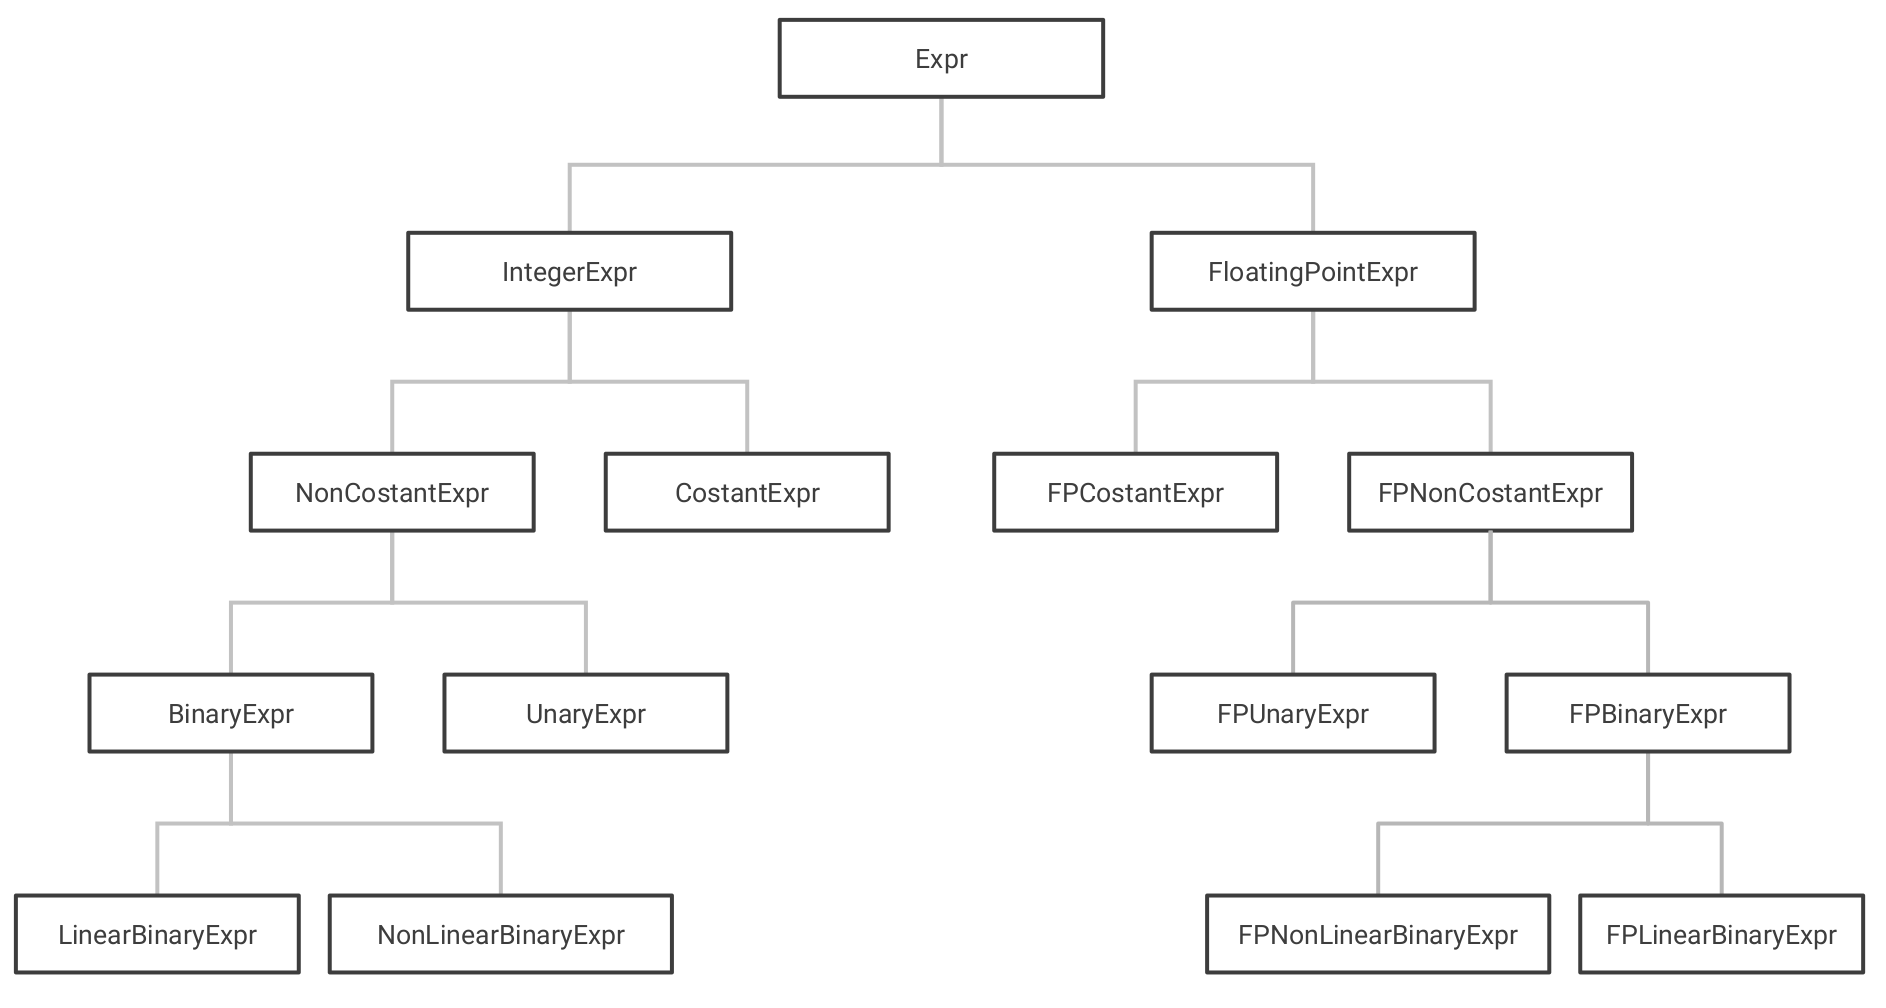
\includegraphics[scale=0.28]{foto/gerarchia.png}
    \caption{Gerarchia delle classi modificata, tutto il ramo destro ad \textit{Expr} è stato aggiunto}
    \label{fig:gerarchia}
\end{figure}




\newpage
Ognuna delle classi derivanti da \textit{IntegerExpr} e \textit{FloatingPointExpr}, a sua volta, definisce le sottoclassi vere e proprie che caratterizzano una certa operazione in ambito simbolico e che conterranno tutte quelle informazioni mostrate ad inizio paragrafo.
\newline \newline
Ad esempio, la classe per la rappresentazione simbolica della Addss è la seguente:
\begin{figure}[h]
\begin{lstlisting}[xleftmargin=0\textwidth, language=SymQEMU, basicstyle=\small]
class AddssExpr : public FPLinearBinaryExpr {
public:
  AddssExpr(ExprRef l, ExprRef h)
    : FPLinearBinaryExpr(Addss, l, h) {}

protected:
  std::string getName() const override {
    return "Addss";
  }

  z3::expr toZ3ExprRecursively(bool verbose) override {
    Z3_ast c0 = children_[0]->toZ3Expr(verbose);
    Z3_ast c1 = children_[1]->toZ3Expr(verbose);
    return c0 + c1;
  }
};
\end{lstlisting}
    \caption{Classe che crea l'espressione simbolica Addss}
    \label{fig:AddssExpr}
\end{figure}
\newline \newline
Dopo aver chiarito la costruzione dell'espressione simbolica tramite le classi, bisogna creare una nuova classe per l'operazione da aggiungere ed associarla alla costruzione di un nuovo oggetto di tipo espressione simbolica.
\newline \newline
Per evitare di scrivere manualmente il codice delle classi nella gerarchia, QSYM utilizza,  ove possibile, uno script Python per generare automaticamente il loro codice C++.
Le nostre modifiche hanno quindi dovuto tener conto di questo generatore.
\newline \newline
QSYM definisce una classe radice \textit{ExprBuilder}, che si occupa di creare gli oggetti delle classi nella gerarchia, è generata in parte dallo script Python prima citato ed è collegata a tutte le sue sottoclassi tramite un puntatore ad una lista.
\newline
Quando viene invocata la costruzione di una nuova espressione simbolica, viene inizialmente eseguito il corpo della funzione associata alla classe radice.
\newline
Dopo aver terminato l'esecuzione di questa, tramite il puntatore alle sottoclassi si va ad invocare nuovamente la medesima funzione relativa però alla successiva sottoclasse, e questo si ripete finché non si arriva all'ultimo elemento della lista.
\newline \newline
Fra le varie sottoclassi di \textit{ExprBuilder}, noi siamo interessati solo alle seguenti due:
\begin{itemize}
    \item \textit{BaseExprBuilder}: è la classe che si preoccupa di costruire, a sua volta, la classe che definisce l'espressione simbolica per una certa operazione, come quella mostrata in Figura (\ref{fig:AddssExpr})
    \item \textit{SymbolicExprBuilder}: è la classe che definisce il comportamento da adottare al variare delle espressioni simboliche ricevute in ingresso.
\end{itemize}





\newpage
In questo studio ci si è concentrati sul fornire il supporto alle operazioni matematiche di base nella forma più semplice possibile, in modo da avere una base da cui partire per ulteriori sviluppi.
\newline \newline
Sapendo adesso il flusso esecutivo compiuto da QSYM per la costruzione di un'espressione simbolica, quello che rimane è la definizione del corpo del metodo di costruzione definito all'interno di SymCC nel runtime di QSYM.
\begin{figure}[h]
\begin{lstlisting}[xleftmargin=0\textwidth, language=SymQEMU, basicstyle=\small]
SymExpr _sym_build_addss(SymExpr a, SymExpr b) { 
    return registerExpression(g_expr_builder->createAddss( 
                allocatedExpressions.at(a), allocatedExpressions.at(b))); 
}
\end{lstlisting}
    \caption{Funzione che invoca il builder globale, il quale a sua volta andrà ad invocare}{la funzione più giusta per la rappresentazione dell'espressione simbolica dell'Addss}
    \label{fig:costruzione_addss}
\end{figure}







\newpage
\section{Utilizzo di Z3}
Come mostrato nella Figura (\ref{fig:AddssExpr}), l'utilizzo della sintassi Z3 avviene nel metodo "toZ3ExprRecursively()" messo a disposizione dalle classi che definiscono le operazioni in modo simbolico.
\newline \newline
Per la rappresentazione simbolica delle operazioni matematiche non è stata inserita alcuna invocazione di funzioni particolari, in quanto i tipi Z3 fanno overloading degli operatori matematici C++.
\newline
Durante però la definizione di altre funzioni di supporto, come ad esempio le operazioni di conversione e confronto per floating-point, è stato necessario costruire esplicitamente l'espressione simbolica corretta tramite i metodi messi a disposizione da Z3.
\newline \newline
Per la conversione int-float, ad esempio, si è utilizzata la seguente funzione:
\newline
\begin{figure}[h]
\vspace{-4.0mm}
\begin{lstlisting}[xleftmargin=0\textwidth, language=SymQEMU, basicstyle=\small]
Z3_sort sort = Z3_mk_fpa_sort(context_, 8, 24); 
Z3_inc_ref(context_, (Z3_ast)sort);
Z3_ast rm = Z3_mk_fpa_rtz(context_);
Z3_inc_ref(context_, rm);
Z3_ast c0 = children_[0]->toZ3Expr(verbose);
Z3_inc_ref(context_, c0);
Z3_ast bv = Z3_mk_fpa_to_fp_signed(context_, rm, c0, sort);
Z3_inc_ref(context_, bv);
z3::expr result = to_expr(context_, bv);
Z3_dec_ref(context_, bv);
Z3_dec_ref(context_, c0);
Z3_dec_ref(context_, rm);
Z3_dec_ref(context_, (Z3_ast)sort);
return result;
\end{lstlisting}
    \caption{Costruzione dell'espressione simbolica per una costante floating-point}
    \label{fig:Cvtsi2ssExpr}
\end{figure}
\ \\
Se analizzata attentamente, è possibile notare l'unione di sintassi C e C++ all'interno della funzione.
\newline
Essendo il runtime di QSYM scritto in C++, le classi definite al suo interno fanno uso delle API messe a disposizione da Z3++, ottenendo un codice più compatto ma anche meno leggibile.
\newline
Studiando però la libreria Z3++, si è scoperto che tutte le API C++ fornite non sono altro che dei wrapper per l'esecuzione di molteplici metodi Z3, pertanto è possibile utilizzare le API C e poi convertire l'espressione generata in una comprensibile a C++ tramite il metodo "to\_expr" di Z3++.
\newline \newline
Un'altra particolarità aggiunta da Z3++, non presente in Z3, è l'inserimento di un nuovo metodo per la gestione dei dati simbolici, che può essere paragonato al medesimo modo in cui un computer memorizza i suoi file tramite \textit{hard-link}.
\newline
Ogni volta che un nuovo dato viene creato, bisogna aumentare il contatore dei riferimenti ad esso tramite "Z3\_inc\_ref()", così come bisogna decrementarlo tramite "Z3\_dec\_ref()" se l'oggetto in questione non viene più utilizzato.
\newline
Se il numero di riferimenti verso un oggetto diventa pari a 0, significa che questo non è più necessario e viene pulita la memoria che vi era stata assegnata.

\newpage
\chapter{Esempi di funzionamento}
\ \\
Prima di passare alla dimostrazione pratica dell'applicazione di SymQEMU su programmi che utilizzano l'aritmetica floating-point, è importante parlare anche di tutte le funzioni di supporto accennate nei capitoli precedenti e necessarie per la corretta costruzione dell'espressione simbolica finale.
\newline \newline
Oltre alle operazioni matematiche di base, sono state implementate anche le seguenti funzioni:
\begin{itemize}
    \item conversione da intero con segno a floating-point a singola precisione
    \item operazione di confronto ordered tra due floating-point
    \item costruzione di una costante floating-point simbolica
\end{itemize}
\ \\
La prima operazione è gestita dall'opcode CVTSI2SS, la cui implementazione risulta essere la seguente:
\begin{figure}[h]
\begin{lstlisting}[xleftmargin=0\textwidth, language=SymQEMU2, basicstyle=\small]
void helper_sym_cvtsi2ss(ZMMReg* dst, void* expr){
    if (expr == NULL)
        _sym_write_memory((uint8_t*)dst, 4*sizeof(int), NULL, true);

    else{
        SymExpr symbolic = _sym_build_cvtsi2ss(expr);
        _sym_write_memory((uint8_t*)dst, sizeof(int), symbolic, true);
    }
}
\end{lstlisting}
    \caption{Corpo dell’helper simbolico per la CVTSI2SS}
    \label{fig:helper_cvtsi2ss}
\end{figure}
\ \\ \newline
Se l'input iniziale è concreto allora viene inizializzata a 0 la memoria simbolica del registro associato, altrimenti l'espressione simbolica ricevuta in ingresso viene messa come parametro di un'altra espressione che provvederà poi a convertirla in floating-point.
\newline\newline
L'operazione di confronto tra floating-point avviene tramite la COMISS, la quale utilizza un metodo di determinazione della relazione d'ordine tra i due operandi diverso da quello più comune, in cui si andrebbe a verificare direttamente il simbolo matematico interessato.
\newline
L'operatore COMISS effettua una serie di controlli in cascata associando ad ognuno di essi una possibile relazione d'ordine tra i due operandi, in modo tale che se una condizione non è soddisfatta, la relazione d'ordine associata non è verificata.
\newline
Dopo aver stabilito la relazione d'ordine corretta, nel registro EFLAGS della CPU viene scritta una particolare sequenza di bit che identifica il risultato ottenuto.




\newpage
Per dare un'idea più chiara del flusso esecutivo, riportiamo l'espressione simbolica generata dal metodo "toZ3ExprRecursively" della classe \textit{ComissExpr}.
\begin{figure}[h]
\begin{lstlisting}[xleftmargin=0\textwidth, language=SymQEMU, basicstyle=\footnotesize]
Z3_sort bv_sort = Z3_mk_bv_sort(context_, 32);
Z3_inc_ref(context_, Z3_ast(bv_sort));
Z3_ast unordered = Z3_mk_numeral(context_, "69", bv_sort); 
Z3_inc_ref(context_, unordered);
Z3_ast maggiore = Z3_mk_numeral(context_, "0", bv_sort);
Z3_inc_ref(context_, maggiore);
Z3_ast uguale = Z3_mk_numeral(context_, "64", bv_sort);
Z3_inc_ref(context_, uguale);
Z3_ast minore = Z3_mk_numeral(context_, "1", bv_sort); 
Z3_inc_ref(context_, minore);

Z3_ast c0 = children_[0]->toZ3Expr(verbose);
Z3_inc_ref(context_, c0);
Z3_ast c1 = children_[1]->toZ3Expr(verbose);
Z3_inc_ref(context_, c1);

Z3_ast if_3 = Z3_mk_ite(context_, Z3_mk_fpa_lt(context_, c0, c1), minore, unordered);    
Z3_inc_ref(context_, if_3);

Z3_ast if_2 = Z3_mk_ite(context_, Z3_mk_fpa_gt(context_, c0, c1), maggiore, uguale);
Z3_inc_ref(context_, if_2);

Z3_ast if_1 = Z3_mk_ite(context_, Z3_mk_fpa_geq(context_, c0, c1), if_2, if_3);
Z3_inc_ref(context_, if_1);
    
z3::expr res = to_expr(context_, if_1);
    
Z3_dec_ref(context_, c0);
Z3_dec_ref(context_, c1);
Z3_dec_ref(context_, Z3_ast(bv_sort));
Z3_dec_ref(context_, unordered);
Z3_dec_ref(context_, maggiore);
Z3_dec_ref(context_, uguale);
Z3_dec_ref(context_, minore);
Z3_dec_ref(context_, if_3);
Z3_dec_ref(context_, if_2);
Z3_dec_ref(context_, if_1);
return res;
\end{lstlisting}
    \caption{Costruzione dell'espressione simbolica per il confronto tra floating-point}
    \label{fig:ComissExpr}
\end{figure}
\ \\ \newline
Nella prima parte della funzione vengono costruite delle variabili rappresentanti le stringhe di bit del registro EFLAGS, che identificano la relazione d'ordine che la destinazione ha rispetto alla sorgente, ed i valori numerici indicati nelle funzioni altro non sono che la conversione in decimale di tale stringa binaria.



\newpage
I controlli in cascata, descritti poco prima, sono eseguiti secondo il seguente ordine:
\begin{itemize}
    \item destinazione $\geq$ sorgente?
    \begin{itemize}
        \item V: destinazione > sorgente?
        \begin{itemize}
            \item V: maggiore
            \item F: uguale
        \end{itemize}
        \item F: destinazione < sorgente?
        \begin{itemize}
            \item V: minore
            \item F: indefinito
        \end{itemize}
    \end{itemize}
\end{itemize}
\ \\
Mettendo questi costrutti condizionali all'interno dell'espressione simbolica, andrà a verificarsi la divisione in due dell'analisi in fase di risoluzione da parte del solver, procedendo così alla scoperta di rami che potrebbero portare alla generazione di nuovi risultati interessanti.
\newline \newline \newline
Infine, l'operazione di costruzione di una costante floating-point simbolica avviene esclusivamente all'interno del runtime di QSYM, agendo come funzione di supporto alla costruzione dell'espressione simbolica finale.
\newline
Partendo da un valore concreto, si estrae il contenuto reale del registro la cui memoria simbolica è stata marcata a 0, e con Z3 si costruisce una variabile che lo rappresenti.
\newline \newline
Questa funzione viene usata, ad esempio, nella Figura (\ref{fig:corpo_sym_addss}) tramite l'invocazione di "\_sym\_build\_floating\_point()", e la classe che la costruisce è la seguente:
\begin{figure}[h]
\begin{lstlisting}[xleftmargin=0\textwidth, language=SymQEMU, basicstyle=\footnotesize]
class FPConstantExpr : public FloatingPointExpr{

public:
  FPConstantExpr(double value, UINT32 bits) :
    FloatingPointExpr(Constant, bits), value_(value), bits_ (bits) {}

protected:
  std::string getName() const override {
    return "Floating-point Constant";
  }

  bool printAux(ostream& os) const override {
    os << "value=" << value_;
    return true;
  }

  z3::expr toZ3ExprRecursively(bool verbose) override {
      if (bits_ == 32)
        return context_.fpa_val((float)value_);
      else
        return context_.fpa_val(value_);
  }

  double value_; 
  int bits_;
};
\end{lstlisting}
    \caption{Classe per la costruzione simbolica di una costante floating-point}
    \label{fig:FPConstantExpr}
\end{figure}
\ \\

\newpage
\section{Analisi del codice utilizzato come esempio}
Lo scheletro del codice utilizzato come base per i test è il seguente:
\begin{figure}[h]
\begin{lstlisting}[xleftmargin=0\textwidth, language=C, basicstyle=\small]
#include <stdio.h>
#include <stdlib.h>
#include <fcntl.h>
#include <unistd.h>

float foo (int a){
    // operazione matematica studiata + costrutto if-else
}

int main (int argc, char* argv[]){
    int desc = open(argv[1], O_RDONLY);
    if (desc == -1){
        return -1;
    }

    int buf;
    int byte_letti = read(desc, &buf, sizeof(int));
    if (byte_letti < 4){
        return -1;
    }

    printf("%f\n", foo(buf));

    if (close(desc) == -1){
        return -1;
    }

    return 0;
}
\end{lstlisting}
    \caption{Codice C per gli esempi, la funzione "foo" varierà a seconda del test effettuato}
    \label{fig:codice_base}
\end{figure}
\ \\ \newline
Partendo dal descrittore verso il file di input fornito da terminale, viene fatta una lettura di 4 byte e scritto il risultato all'interno di buf, il quale sarà poi passato come parametro alla funzione "foo".
\newline
All'interno di questa verrà effettuata un'operazione matematica tra il valore intero in ingresso ed uno floating-point costante, portando quindi all'esecuzione prima di una conversione (CVTSI2SS) e successivamente del calcolo, ed il risultato verrà confrontato con un altro valore floating-point costante (COMISS) e restituito un generico valore di ritorno.
\newline \newline
L'esecuzione del progetto avviene in due fasi:
\begin{itemize}
    \item la prima consiste nell'esecuzione del codice binario da parte di SymQEMU, in cui andremo sempre a specificare da terminale un file "input.dat" da cui effettuare la lettura simbolica, ed il cui contenuto sarà analizzato in seguito
    \item la seconda consiste, invece, nel testare i nuovi input generati a seguito dell'analisi, e questo viene fatto lanciando da terminale il solo codice binario e specificando i nuovi input generati come file da cui leggere
\end{itemize}




\newpage
Il file "input.dat" contiene 4 byte composti interamente da soli zeri, pertanto non è normalmente stampabile da un editor di testo, e per leggerne il contenuto è necessario effettuare un \textit{hexdump} del file:
\begin{lstlisting}[xleftmargin=0\textwidth, language=bash]
$ xxd input.dat
00000000: 0000 0000         ....
\end{lstlisting}
\ \\
Il comando "xxd" mostra il contenuto del file nel seguente modo:
\begin{itemize}
    \item la colonna a sinistra mostra il byte da cui parte l'offset del cursore per la lettura, e nel nostro caso è composta da soli zeri perché l'inizio del file
    \item nella colonna centrale sono presenti i byte che compongono effettivamente il file, rappresentati in notazione esadecimale, da leggere a coppie di due partendo da sinistra
    \item nella colonna a destra è presente la rappresentazione in ASCII dei byte mostrati, se possibile, altrimenti viene inserito il simbolo "."
\end{itemize}
\ \\
Per garantire inoltre il corretto funzionamento dell'esecutore simbolico, SymQEMU richiede che vengano definite delle variabili globali nell'ambiente di esecuzione: una contiene il percorso assoluto al file di input, il cui contenuto sarà letto ed interpretato come dati simbolici, mentre l'altra contiene il percorso assoluto alla cartella in cui scrivere i file generati a seguito dell'analisi.
\newline \newline \newline
Il codice mostrato in Figura (\ref{fig:codice_base}), il file "input.dat" e le variabili globali appena descritte rimarranno costanti in tutti gli esempi mostrati in seguito, le uniche variabili saranno il contenuto della funzione "foo" ed il nome del file generato da SymQEMU a seguito dell'analisi poiché non può essere predetto.







\newpage
\section{Esempio 1: Somma}
Nel test per l'operazione ADDSS è stato usato il seguente codice:
\newline
\begin{lstlisting}[xleftmargin=0\textwidth, language=C, basicstyle=\small]
#include <stdio.h>
#include <stdlib.h>
#include <fcntl.h>
#include <unistd.h>

float foo (int a){
    float x = 13.89;
    float res = x + a;
    if (res < 123.45f)
        return 1.0;
    else 
        return -1.0;
}

int main (int argc, char* argv[]){
    int desc = open(argv[1], O_RDONLY);
    if (desc == -1){
        return -1;
    }

    int buf;
    int byte_letti = read(desc, &buf, sizeof(int));
    if (byte_letti < 4){
        return -1;
    }

    printf("%f\n", foo(buf));

    if (close(desc) == -1){
        return -1;
    }

    return 0;
}
\end{lstlisting}
\ \\ \newline
Avviando SymQEMU tramite terminale, otteniamo il seguente risultato:
\begin{lstlisting}[xleftmargin=0\textwidth, basicstyle=\footnotesize]
$ export SYMCC_INPUT_FILE=/home/user/progetto_laurea/codice/input/input.dat

$ export SYMCC_OUTPUT_DIR=/home/user/progetto_laurea/codice/risultati/

$ /home/user/symqemu/BUILD/x86_64-linux-user/symqemu-x86_64  ./test_file 
  /home/user/progetto_laurea/codice/input/input.dat

This is SymCC running with the QSYM backend
Making data read from /home/user/progetto_laurea/codice/input/input.dat as symbolic
[STAT] SMT: { "solving_time": 0, "total_time": 80929 }
[STAT] SMT: { "solving_time": 90797 }
[INFO] New testcase: /home/user/progetto_laurea/codice/risultati/000000

1.000000
\end{lstlisting}




\newpage
Analizzando attentamente l'output possiamo ricavare importanti informazioni.
\newline \newline
Innanzitutto, il componente di SymCC riutilizzato da SymQEMU  ha letto il contenuto del file "input.dat", andando ad interpretarne il contenuto in modo simbolico.
\newline
Successivamente l'SMT solver mostra informazioni temporali circa l'espressione simbolica da noi generata, indicando prima il tempo impiegato dal solver e dopo quello impiegato complessivamente per l'analisi.
\newline
Inoltre l'analisi ha generato un nuovo input interessante, che è stato scritto all'interno del file "000000" e posto nella cartella di output.
\newline
Infine, il valore finale "1.000000" è il risultato della stampa del codice da noi scritto, mostrando quindi che l'esecuzione iniziale ha verificato la condizione della if all'interno della funzione "foo".
\newline \newline 
Se analizzato il nuovo file tramite \textit{hexdump}, troviamo il seguente contenuto:
\begin{lstlisting}[xleftmargin=0\textwidth, language=bash]
$ xxd ./risultati/000000
00000000: d304 7f0e         ....
\end{lstlisting}
Effettuando poi la conversione in decimale del valore mostrato sopra, il nuovo caso generato dal solver è pari a $3540287246$.
\newline \newline
Se adesso lanciassimo il codice tramite terminale, specificando come file di input il nuovo caso generato, otteniamo il seguente risultato:
\begin{lstlisting}[xleftmargin=0\textwidth, language=bash]
$ ./test_file ./risultati/000000

-1.00000
\end{lstlisting}
\ \\
Il nuovo risultato generato da SymQEMU contiene un valore che ha consentito l'esplorazione del ramo della if opposto a quello inizialmente eseguito, pertanto è stato generato un input interessante che ha portato a scoprire un nuovo comportamento del programma.








\newpage
\section{Esempio 2: Sottrazione}
Nel test per l'operazione SUBSS è stato usato il seguente codice:
\newline
\begin{lstlisting}[xleftmargin=0\textwidth, language=C, basicstyle=\small]
#include <stdio.h>
#include <stdlib.h>
#include <fcntl.h>
#include <unistd.h>

float foo (int a){
    float x = 15.5;
    float res = x - a;
    if (res > 10.0f)
        return 1.0;
    else 
        return -1.0;
}

int main (int argc, char* argv[]){
    int desc = open(argv[1], O_RDONLY);
    if (desc == -1){
        return -1;
    }

    int buf;
    int byte_letti = read(desc, &buf, sizeof(int));
    if (byte_letti < 4){
        return -1;
    }

    printf("%f\n", foo(buf));

    if (close(desc) == -1){
        return -1;
    }

    return 0;
}
\end{lstlisting}
\ \\ \newline
Avviando SymQEMU tramite terminale, otteniamo il seguente risultato:
\begin{lstlisting}[xleftmargin=0\textwidth, basicstyle=\footnotesize]
$ export SYMCC_INPUT_FILE=/home/user/progetto_laurea/codice/input/input.dat

$ export SYMCC_OUTPUT_DIR=/home/user/progetto_laurea/codice/risultati/

$ /home/user/symqemu/BUILD/x86_64-linux-user/symqemu-x86_64  ./test_file 
  /home/user/progetto_laurea/codice/input/input.dat

This is SymCC running with the QSYM backend
Making data read from /home/user/progetto_laurea/codice/input/input.dat as symbolic
[STAT] SMT: { "solving_time": 0, "total_time": 67886 }
[STAT] SMT: { "solving_time": 41244 }
[INFO] New testcase: /home/user/progetto_laurea/codice/risultati/000000

1.000000
\end{lstlisting}


\newpage
Analizzando il nuovo file tramite \textit{hexdump}, otteniamo il seguente risultato:
\begin{lstlisting}[xleftmargin=0\textwidth, language=bash]
$ xxd ./risultati/000000
00000000: 1200 0000         ....
\end{lstlisting}
Convertendo in decimale tale numero si ottiene $301989888$.
\newline \newline
Lanciando il codice sul file di input con il nuovo caso generato, viene restituito quanto segue:
\begin{lstlisting}[xleftmargin=0\textwidth, language=bash]
$ ./test_file ./risultati/000000

-1.00000
\end{lstlisting}






\newpage
\section{Esempio 3: Moltiplicazione}
Nel test per l'operazione MULSS è stato usato il seguente codice:
\newline
\begin{lstlisting}[xleftmargin=0\textwidth, language=C, basicstyle=\small]
#include <stdio.h>
#include <stdlib.h>
#include <fcntl.h>
#include <unistd.h>

float foo (int a){
    float x = 48.1475;
    float res = x * a;
    if (res < 503.2485f)
        return 1.0;
    else 
        return -1.0;
}

int main (int argc, char* argv[]){
    int desc = open(argv[1], O_RDONLY);
    if (desc == -1){
        return -1;
    }

    int buf;
    int byte_letti = read(desc, &buf, sizeof(int));
    if (byte_letti < 4){
        return -1;
    }

    printf("%f\n", foo(buf));

    if (close(desc) == -1){
        return -1;
    }

    return 0;
}
\end{lstlisting}
\ \\ \newline
Avviando SymQEMU tramite terminale, otteniamo il seguente risultato:
\begin{lstlisting}[xleftmargin=0\textwidth, basicstyle=\footnotesize]
$ export SYMCC_INPUT_FILE=/home/user/progetto_laurea/codice/input/input.dat

$ export SYMCC_OUTPUT_DIR=/home/user/progetto_laurea/codice/risultati/

$ /home/user/symqemu/BUILD/x86_64-linux-user/symqemu-x86_64  ./test_file 
  /home/user/progetto_laurea/codice/input/input.dat

This is SymCC running with the QSYM backend
Making data read from /home/user/progetto_laurea/codice/input/input.dat as symbolic
[STAT] SMT: { "solving_time": 0, "total_time": 71333 }
[STAT] SMT: { "solving_time": 81006 }
[INFO] New testcase: /home/user/progetto_laurea/codice/risultati/000000

1.000000
\end{lstlisting}


\newpage
Il risultato generato, se analizzato tramite \textit{hexdump}, è il seguente:
\begin{lstlisting}[xleftmargin=0\textwidth, language=bash]
$ xxd ./risultati/000000
00000000: 9d1c 013c         ....
\end{lstlisting}
Dopo aver convertito in decimale, otteniamo il valore $2635858236$.
\newline \newline
Eseguendo il codice da terminale con parametro di input il nuovo caso generato, si ottiene:
\begin{lstlisting}[xleftmargin=0\textwidth, language=bash]
$ ./test_file ./risultati/000000

-1.00000
\end{lstlisting}








\newpage
\section{Esempio 4: Divisione}
Nel test per l'operazione DIVSS è stato usato il seguente codice:
\newline
\begin{lstlisting}[xleftmargin=0\textwidth, language=C, basicstyle=\small]
#include <stdio.h>
#include <stdlib.h>
#include <fcntl.h>
#include <unistd.h>

float foo (int a){
    float x = 456.789;
    float res = x / a;
    if (res < 1.23f)
        return 1.0;
    else 
        return -1.0;
}

int main (int argc, char* argv[]){
    int desc = open(argv[1], O_RDONLY);
    if (desc == -1){
        return -1;
    }

    int buf;
    int byte_letti = read(desc, &buf, sizeof(int));
    if (byte_letti < 4){
        return -1;
    }

    printf("%f\n", foo(buf));

    if (close(desc) == -1){
        return -1;
    }

    return 0;
}
\end{lstlisting}
\ \\ \newline
Avviando SymQEMU tramite terminale, otteniamo il seguente risultato:
\begin{lstlisting}[xleftmargin=0\textwidth, basicstyle=\footnotesize]
$ export SYMCC_INPUT_FILE=/home/user/progetto_laurea/codice/input/input.dat

$ export SYMCC_OUTPUT_DIR=/home/user/progetto_laurea/codice/risultati/

$ /home/user/symqemu/BUILD/x86_64-linux-user/symqemu-x86_64  ./test_file 
  /home/user/progetto_laurea/codice/input/input.dat

This is SymCC running with the QSYM backend
Making data read from /home/user/progetto_laurea/codice/input/input.dat as symbolic
[STAT] SMT: { "solving_time": 0, "total_time": 67014 }
[STAT] SMT: { "solving_time": 363044 }
[INFO] New testcase: /home/user/progetto_laurea/codice/risultati/000000

-1.000000
\end{lstlisting}






\newpage
L'output ottenuto, scomposto tramite \textit{hexdump}, è mostrato di seguito:
\begin{lstlisting}[xleftmargin=0\textwidth, language=bash]
$ xxd ./risultati/000000
00000000: 116c f7f7         ....
\end{lstlisting}
Il risultato ottenuto, se riportato in forma decimale, equivale a $292354039$.
\newline \newline
Mandando in esecuzione il codice facendo uso del nuovo caso generato come file di input, si ottiene:
\begin{lstlisting}[xleftmargin=0\textwidth, language=bash]
$ ./test_file ./risultati/000000

1.00000
\end{lstlisting}












\chapter{Conclusioni}
\ \\
Inizialmente, gli obiettivi finali di questa tesi erano lo studio di \textit{symbolic execution} e l'implementazione della funzione di somma floating-point all'interno dell'esecutore concolico SymQEMU.
\newline \newline
Per fare ciò si è partiti dall'effettuare un'approfondita analisi dell'esecutore fornito, studiandone il flusso esecutivo attraverso i vari framework da cui è costituito, cercando di ottenere un livello di conoscenza del codice sufficiente affinché vi si potessero implementare nuove operazioni.
\newline
Successivamente, è stato necessario studiare il comportamento adottato dal compilatore \textit{gcc} da noi usato per la generazione degli eseguibili, e questo perché le scelte progettuali adottate per la costruzione del file binario avrebbero determinato gli opcode da implementare simbolicamente.
\newline
Infine, poiché le espressioni simboliche generate dovranno essere processate da un solver, sono stati creati svariati codici di test al fine di comprendere il corretto funzionamento dell'SMT solver Z3, prendendo dimestichezza con la libreria fornita per la costruzione simbolica e dei metodi utilizzati per la risoluzione delle formule generate.
\newline \newline
Dopo aver concluso la fase preparatoria, ottenuto conoscenze sufficienti sulle istruzioni interessanti, compreso come inserirle nel runtime di SymQEMU ed infine costruirle simbolicamente con Z3, si è passati all'implementazione vera e propria all'interno dell'esecutore.
\newline \newline
L'implementazione parte dal runtime di SymQEMU, in cui si è andati a modificare il file di traduzione delle istruzioni Intel x86 e x86\_64 messo a disposizione da QEMU, inserendo l'invocazione di un helper simbolico da noi costruito per la gestione dell'operazione ADDSS.
\newline
Dopo aver definito l'intestazione dell'helper, specificando il tipo dei parametri inseriti e l'eventuale tipo di ritorno, si è passati a definirne il corpo, contenente tutti i metodi per la corretta lettura e scrittura della memoria simbolica al fine di ottenere due espressioni simboliche pronte ad essere combinate tra loro.
\newline
Le espressioni simboliche prima descritte passano al runtime di SymCC, dove viene allocata memoria per la loro gestione e preparate all'utilizzo da parte di QSYM.
\newline
Partendo da un costruttore simbolico globale, viene costruita la classe più adatta per rappresentare l'operazione simbolica di somma floating-point all'interno del runtime di QSYM, la quale conterrà tutte le informazioni necessarie alla sua definizione ed il metodo che andrà a costruire tramite la libreria Z3 l'espressione finale processata dal solver.
\newline \newline
Una volta assicuratosi che la funzione ADDSS fosse stata implementata simbolicamente all'interno di SymQEMU e che la generazione di nuovi input avvenisse in modo corretto, il processo appena mostrato è stato replicato per l'inserimento delle altre operazioni matematiche di base, ovvero prodotto, divisione e differenza.




\newpage
\section{Considerazioni finali e lavoro futuro}
Questo studio si è voluto concentrare sull'implementazione delle operazioni aritmetiche floating-point più semplici, limitandosi ai quattro operatori matematici di base, e definendo anche tutte le funzioni di supporto necessarie alla corretta costruzione dell'espressione simbolica finale.
\newline
Nonostante il lavoro svolto rappresenti il minimo indispensabile necessario per la corretta analisi di una espressione floating-point, costituisce comunque una base da cui poter partire per l'aggiunta di tutte le altre operazioni messe a disposizione dal set di istruzioni SSE/SSE2 con un basso sforzo implementativo.
\newline \newline
Discorso più complesso si ha, invece, nel caso del set di istruzioni x87 utilizzato dalla FPU e della doppia precisione estesa.
\newline \newline
Come accennato nel paragrafo 3.2, la doppia precisione estesa prevede uno speciale bit di controllo all'interno della sequenza che può cambiarne l'intero significato, partendo da un numero \textit{denormal} ad uno potenzialmente infinito o addirittura NaN.
\newline
Durante la fase di studio di SymQEMU sono state anche analizzate le scelte progettuali fatte dagli sviluppatori in merito proprio alla gestione di questi numeri speciali, che nel corso della tesi non abbiamo riportato per questioni di semplicità, e che consentirebbero un'implementazione corretta dell'utilizzo della FPU ma ad un costo troppo elevato in termini di precisione.
\newline
Per evitare di dover gestire le eventuali eccezioni generate dalla CPU a seguito dell'esecuzione di operazioni matematiche floating-point con numeri speciali, SymQEMU implementa delle semplificazioni eccessive, eliminando alla radice potenziali valori scomodi che impedirebbero una corretta analisi dell'espressione simbolica finale.
\newline
Un esempio risulta essere la gestione dei numeri \textit{denormal}, numeri infinitesimi il cui numero di zeri che precede la prima cifra significativa eccede quelli rappresentabili dall'esponente utilizzato, e che SymQEMU invece elimina, portando direttamente a zero l'intera regione di memoria assegnata per la rappresentazione e quindi annullandone completamente il valore.
\newline \newline
In merito all'aggiunta del set di istruzioni x87 e la gestione dei registri ST(i) a stack usati dalla FPU, sosteniamo che il flusso implementativo mostrato per le istruzioni SSE/SSE2 possa essere riapplicato nella sua interezza, facendo però attenzione al nuovo comportamento a stack FIFO dei registri.



\backmatter
\phantomsection
\begin{thebibliography}{0}

\bibitem{ref:survey}
Roberto Baldoni, Emilio Coppa, Daniele Cono D'Elia, Camil Demetrescu, and Irene Finocchi, "\textit{A Survey of Symbolic Execution Techniques}", ACM Computer Surveys, 2018
\newline
\url{https://arxiv.org/pdf/1610.00502.pdf}

\bibitem{ref:symqemu}
Sebastian Poeplau and Aurelien Francillon, "\textit{SymQEMU:
Compilation-based symbolic execution for binaries}", Network and Distributed System Security Symposium, February 2021
\newline
\url{http://www.s3.eurecom.fr/docs/ndss21_symqemu.pdf}

\bibitem{ref:symcc}
Sebastian Poeplau and Aurelien Francillon, "\textit{Symbolic execution with SYMCC: Don’t interpret, compile!}",USENIX Association, August 2020
\newline
\url{http://www.s3.eurecom.fr/docs/usenixsec20_symcc.pdf}

\bibitem{ref:qsym}
Insu Yun, Sangho Lee, Meng Xu, Yeongjin Jang and Taesoo Kim ,"\textit{Qsym: A Practical Concolic Execution Engine Tailored for Hybrid Fuzzing}", 27th USENIX Security Symposium (USENIX Security 18), August 2018
\newline
\url{https://www.usenix.org/system/files/conference/usenixsecurity18/sec18-yun.pdf}

\bibitem{ref:z3}
Nikolaj Bjørner, Leonardo de Moura, Lev Nachmanson, and Christoph Wintersteiger, "\textit{Z3: An Efficient SMT solver}", Microsoft Research, 2008
\newline
\url{https://nikolajbjorner.github.io/slides/Z3_System.pdf}

\bibitem{ref:float}
Wikimedia Commons, "\textit{The memory format of an IEEE 754 single-precision floating-point value}",
\url{http://en.wikipedia.org/wiki/Single-precision_floating-point_format}

\bibitem{ref:double}
Wikimedia Commons, "\textit{The memory format of an IEEE 754 double-precision floating-point value}", 
\url{https://en.wikipedia.org/wiki/Double-precision_floating-point_format}

\bibitem{ref:manuale_intel_1}
"\textit{Intel 64 and IA-32 Architectures Software Developer's Manual, Volume 1: Basic Architecture}", Aprile 2021

\bibitem{ref:80_bit}
Wikimedia Commons, "\textit{The memory format of an IEEE 754 extended-precision floating-point value}"
\newline
\url{https://en.wikipedia.org/wiki/Extended_precision}



\end{thebibliography}



\begin{acknowledgments}
Vorrei utilizzare questo spazio per ringraziare le persone che mi hanno concesso di arrivare alla stesura di questo elaborato.
\newline \newline
Innanzitutto, vorrei ringraziare il mio relatore, il professor Emilio Coppa, per avermi proposto questo progetto e consentito di analizzare la mia passione per l'informatica da un punto di vista completamente nuovo ed affascinante. 
\newline
Le conoscenze da lui fornitemi sono state un elemento fondamentale per la realizzazione della tesi.
\newline \newline
Un ringraziamento speciale va ai miei genitori, che mi hanno reso possibile intraprendere questo percorso riponendo cieca fiducia in me e nelle mie abilità.
\newline
Tutte le ansie e le preoccupazioni di questi ultimi anni sono culminate in un lavoro che non sarebbe mai stato possibile se non aveste creduto in me fin dall'inizio, e per questo ve ne sarò sempre grato.
\newline
Questa laurea è anche vostra, per tutti i sacrifici che avete compiuto per me, e che spero oggi possiate essere felici.
\newline \newline
Ringrazio con tutto il mio cuore Elena, la persona più bella e fantastica che potessi mai immaginare di trovare al mio fianco.
\newline
Il tuo amore coraggioso e forte mi ha dato l’energia e l’entusiasmo che mi hanno permesso di stringere i denti durante ogni avversità e raggiungere finalmente questo traguardo, e non potrò mai ringraziarti abbastanza per tutto il supporto ed il sostegno che mi hai dato durante questo arco della mia vita.
\newline
Sei la mia roccia, la mia ancora, la mia forza. Ti amo.
\newline \newline
Infine, vorrei ringraziare tutti i miei amici: quelli che conosco da una vita, le persone incontrate durante il cammino, quelli vicini e quelli lontani.
\newline
Senza le risate, le ore passate a chiacchierare insieme, le consulenze da ansia pre-esame e post-esame e tutti gli altri bei momenti passati assieme, questo percorso sarebbe stato sicuramente molto più noioso e meno divertente.
\newline
Un grazie va anche a voi, per aver rallegrato le mie giornate ed alleviato il mio animo grazie alle vostre parole.
\end{acknowledgments}


\end{document}